% CVPR 2022 Paper Template
% based on the CVPR template provided by Ming-Ming Cheng (https://github.com/MCG-NKU/CVPR_Template)
% modified and extended by Stefan Roth (stefan.roth@NOSPAMtu-darmstadt.de)

\documentclass[10pt,twocolumn,letterpaper]{article}

%%%%%%%%% PAPER TYPE  - PLEASE UPDATE FOR FINAL VERSION
\usepackage[review]{cvpr}      % To produce the REVIEW version
%\usepackage{cvpr}              % To produce the CAMERA-READY version
%\usepackage[pagenumbers]{cvpr} % To force page numbers, e.g. for an arXiv version

% Include other packages here, before hyperref.
\usepackage{graphicx}
\usepackage{amsmath}
\usepackage{amssymb}
\usepackage{booktabs}

\usepackage{microtype}
\usepackage{xcolor}
\newcommand{\oo}[1]{\textcolor{orange}{#1}}
%%%%% NEW MATH DEFINITIONS %%%%%

\usepackage{amsmath,amsfonts,bm}

% Mark sections of captions for referring to divisions of figures
\newcommand{\figleft}{{\em (Left)}}
\newcommand{\figcenter}{{\em (Center)}}
\newcommand{\figright}{{\em (Right)}}
\newcommand{\figtop}{{\em (Top)}}
\newcommand{\figbottom}{{\em (Bottom)}}
\newcommand{\captiona}{{\em (a)}}
\newcommand{\captionb}{{\em (b)}}
\newcommand{\captionc}{{\em (c)}}
\newcommand{\captiond}{{\em (d)}}

% Highlight a newly defined term
\newcommand{\newterm}[1]{{\bf #1}}


% Figure reference, lower-case.
\def\figref#1{figure~\ref{#1}}
% Figure reference, capital. For start of sentence
\def\Figref#1{Figure~\ref{#1}}
\def\twofigref#1#2{figures \ref{#1} and \ref{#2}}
\def\quadfigref#1#2#3#4{figures \ref{#1}, \ref{#2}, \ref{#3} and \ref{#4}}
% Section reference, lower-case.
\def\secref#1{section~\ref{#1}}
% Section reference, capital.
\def\Secref#1{Section~\ref{#1}}
% Reference to two sections.
\def\twosecrefs#1#2{sections \ref{#1} and \ref{#2}}
% Reference to three sections.
\def\secrefs#1#2#3{sections \ref{#1}, \ref{#2} and \ref{#3}}
% Reference to an equation, lower-case.
\def\eqref#1{equation~\ref{#1}}
% Reference to an equation, upper case
\def\Eqref#1{Equation~\ref{#1}}
% A raw reference to an equation---avoid using if possible
\def\plaineqref#1{\ref{#1}}
% Reference to a chapter, lower-case.
\def\chapref#1{chapter~\ref{#1}}
% Reference to an equation, upper case.
\def\Chapref#1{Chapter~\ref{#1}}
% Reference to a range of chapters
\def\rangechapref#1#2{chapters\ref{#1}--\ref{#2}}
% Reference to an algorithm, lower-case.
\def\algref#1{algorithm~\ref{#1}}
% Reference to an algorithm, upper case.
\def\Algref#1{Algorithm~\ref{#1}}
\def\twoalgref#1#2{algorithms \ref{#1} and \ref{#2}}
\def\Twoalgref#1#2{Algorithms \ref{#1} and \ref{#2}}
% Reference to a part, lower case
\def\partref#1{part~\ref{#1}}
% Reference to a part, upper case
\def\Partref#1{Part~\ref{#1}}
\def\twopartref#1#2{parts \ref{#1} and \ref{#2}}

\def\ceil#1{\lceil #1 \rceil}
\def\floor#1{\lfloor #1 \rfloor}
\def\1{\bm{1}}
\newcommand{\train}{\mathcal{D}}
\newcommand{\valid}{\mathcal{D_{\mathrm{valid}}}}
\newcommand{\test}{\mathcal{D_{\mathrm{test}}}}

\def\eps{{\epsilon}}


% Random variables
\def\reta{{\textnormal{$\eta$}}}
\def\ra{{\textnormal{a}}}
\def\rb{{\textnormal{b}}}
\def\rc{{\textnormal{c}}}
\def\rd{{\textnormal{d}}}
\def\re{{\textnormal{e}}}
\def\rf{{\textnormal{f}}}
\def\rg{{\textnormal{g}}}
\def\rh{{\textnormal{h}}}
\def\ri{{\textnormal{i}}}
\def\rj{{\textnormal{j}}}
\def\rk{{\textnormal{k}}}
\def\rl{{\textnormal{l}}}
% rm is already a command, just don't name any random variables m
\def\rn{{\textnormal{n}}}
\def\ro{{\textnormal{o}}}
\def\rp{{\textnormal{p}}}
\def\rq{{\textnormal{q}}}
\def\rr{{\textnormal{r}}}
\def\rs{{\textnormal{s}}}
\def\rt{{\textnormal{t}}}
\def\ru{{\textnormal{u}}}
\def\rv{{\textnormal{v}}}
\def\rw{{\textnormal{w}}}
\def\rx{{\textnormal{x}}}
\def\ry{{\textnormal{y}}}
\def\rz{{\textnormal{z}}}

% Random vectors
\def\rvepsilon{{\mathbf{\epsilon}}}
\def\rvtheta{{\mathbf{\theta}}}
\def\rva{{\mathbf{a}}}
\def\rvb{{\mathbf{b}}}
\def\rvc{{\mathbf{c}}}
\def\rvd{{\mathbf{d}}}
\def\rve{{\mathbf{e}}}
\def\rvf{{\mathbf{f}}}
\def\rvg{{\mathbf{g}}}
\def\rvh{{\mathbf{h}}}
\def\rvu{{\mathbf{i}}}
\def\rvj{{\mathbf{j}}}
\def\rvk{{\mathbf{k}}}
\def\rvl{{\mathbf{l}}}
\def\rvm{{\mathbf{m}}}
\def\rvn{{\mathbf{n}}}
\def\rvo{{\mathbf{o}}}
\def\rvp{{\mathbf{p}}}
\def\rvq{{\mathbf{q}}}
\def\rvr{{\mathbf{r}}}
\def\rvs{{\mathbf{s}}}
\def\rvt{{\mathbf{t}}}
\def\rvu{{\mathbf{u}}}
\def\rvv{{\mathbf{v}}}
\def\rvw{{\mathbf{w}}}
\def\rvx{{\mathbf{x}}}
\def\rvy{{\mathbf{y}}}
\def\rvz{{\mathbf{z}}}

% Elements of random vectors
\def\erva{{\textnormal{a}}}
\def\ervb{{\textnormal{b}}}
\def\ervc{{\textnormal{c}}}
\def\ervd{{\textnormal{d}}}
\def\erve{{\textnormal{e}}}
\def\ervf{{\textnormal{f}}}
\def\ervg{{\textnormal{g}}}
\def\ervh{{\textnormal{h}}}
\def\ervi{{\textnormal{i}}}
\def\ervj{{\textnormal{j}}}
\def\ervk{{\textnormal{k}}}
\def\ervl{{\textnormal{l}}}
\def\ervm{{\textnormal{m}}}
\def\ervn{{\textnormal{n}}}
\def\ervo{{\textnormal{o}}}
\def\ervp{{\textnormal{p}}}
\def\ervq{{\textnormal{q}}}
\def\ervr{{\textnormal{r}}}
\def\ervs{{\textnormal{s}}}
\def\ervt{{\textnormal{t}}}
\def\ervu{{\textnormal{u}}}
\def\ervv{{\textnormal{v}}}
\def\ervw{{\textnormal{w}}}
\def\ervx{{\textnormal{x}}}
\def\ervy{{\textnormal{y}}}
\def\ervz{{\textnormal{z}}}

% Random matrices
\def\rmA{{\mathbf{A}}}
\def\rmB{{\mathbf{B}}}
\def\rmC{{\mathbf{C}}}
\def\rmD{{\mathbf{D}}}
\def\rmE{{\mathbf{E}}}
\def\rmF{{\mathbf{F}}}
\def\rmG{{\mathbf{G}}}
\def\rmH{{\mathbf{H}}}
\def\rmI{{\mathbf{I}}}
\def\rmJ{{\mathbf{J}}}
\def\rmK{{\mathbf{K}}}
\def\rmL{{\mathbf{L}}}
\def\rmM{{\mathbf{M}}}
\def\rmN{{\mathbf{N}}}
\def\rmO{{\mathbf{O}}}
\def\rmP{{\mathbf{P}}}
\def\rmQ{{\mathbf{Q}}}
\def\rmR{{\mathbf{R}}}
\def\rmS{{\mathbf{S}}}
\def\rmT{{\mathbf{T}}}
\def\rmU{{\mathbf{U}}}
\def\rmV{{\mathbf{V}}}
\def\rmW{{\mathbf{W}}}
\def\rmX{{\mathbf{X}}}
\def\rmY{{\mathbf{Y}}}
\def\rmZ{{\mathbf{Z}}}

% Elements of random matrices
\def\ermA{{\textnormal{A}}}
\def\ermB{{\textnormal{B}}}
\def\ermC{{\textnormal{C}}}
\def\ermD{{\textnormal{D}}}
\def\ermE{{\textnormal{E}}}
\def\ermF{{\textnormal{F}}}
\def\ermG{{\textnormal{G}}}
\def\ermH{{\textnormal{H}}}
\def\ermI{{\textnormal{I}}}
\def\ermJ{{\textnormal{J}}}
\def\ermK{{\textnormal{K}}}
\def\ermL{{\textnormal{L}}}
\def\ermM{{\textnormal{M}}}
\def\ermN{{\textnormal{N}}}
\def\ermO{{\textnormal{O}}}
\def\ermP{{\textnormal{P}}}
\def\ermQ{{\textnormal{Q}}}
\def\ermR{{\textnormal{R}}}
\def\ermS{{\textnormal{S}}}
\def\ermT{{\textnormal{T}}}
\def\ermU{{\textnormal{U}}}
\def\ermV{{\textnormal{V}}}
\def\ermW{{\textnormal{W}}}
\def\ermX{{\textnormal{X}}}
\def\ermY{{\textnormal{Y}}}
\def\ermZ{{\textnormal{Z}}}

% Vectors
\def\vzero{{\bm{0}}}
\def\vone{{\bm{1}}}
\def\vmu{{\bm{\mu}}}
\def\vtheta{{\bm{\theta}}}
\def\va{{\bm{a}}}
\def\vb{{\bm{b}}}
\def\vc{{\bm{c}}}
\def\vd{{\bm{d}}}
\def\ve{{\bm{e}}}
\def\vf{{\bm{f}}}
\def\vg{{\bm{g}}}
\def\vh{{\bm{h}}}
\def\vi{{\bm{i}}}
\def\vj{{\bm{j}}}
\def\vk{{\bm{k}}}
\def\vl{{\bm{l}}}
\def\vm{{\bm{m}}}
\def\vn{{\bm{n}}}
\def\vo{{\bm{o}}}
\def\vp{{\bm{p}}}
\def\vq{{\bm{q}}}
\def\vr{{\bm{r}}}
\def\vs{{\bm{s}}}
\def\vt{{\bm{t}}}
\def\vu{{\bm{u}}}
\def\vv{{\bm{v}}}
\def\vw{{\bm{w}}}
\def\vx{{\bm{x}}}
\def\vy{{\bm{y}}}
\def\vz{{\bm{z}}}

% Elements of vectors
\def\evalpha{{\alpha}}
\def\evbeta{{\beta}}
\def\evepsilon{{\epsilon}}
\def\evlambda{{\lambda}}
\def\evomega{{\omega}}
\def\evmu{{\mu}}
\def\evpsi{{\psi}}
\def\evsigma{{\sigma}}
\def\evtheta{{\theta}}
\def\eva{{a}}
\def\evb{{b}}
\def\evc{{c}}
\def\evd{{d}}
\def\eve{{e}}
\def\evf{{f}}
\def\evg{{g}}
\def\evh{{h}}
\def\evi{{i}}
\def\evj{{j}}
\def\evk{{k}}
\def\evl{{l}}
\def\evm{{m}}
\def\evn{{n}}
\def\evo{{o}}
\def\evp{{p}}
\def\evq{{q}}
\def\evr{{r}}
\def\evs{{s}}
\def\evt{{t}}
\def\evu{{u}}
\def\evv{{v}}
\def\evw{{w}}
\def\evx{{x}}
\def\evy{{y}}
\def\evz{{z}}

% Matrix
\def\mA{{\bm{A}}}
\def\mB{{\bm{B}}}
\def\mC{{\bm{C}}}
\def\mD{{\bm{D}}}
\def\mE{{\bm{E}}}
\def\mF{{\bm{F}}}
\def\mG{{\bm{G}}}
\def\mH{{\bm{H}}}
\def\mI{{\bm{I}}}
\def\mJ{{\bm{J}}}
\def\mK{{\bm{K}}}
\def\mL{{\bm{L}}}
\def\mM{{\bm{M}}}
\def\mN{{\bm{N}}}
\def\mO{{\bm{O}}}
\def\mP{{\bm{P}}}
\def\mQ{{\bm{Q}}}
\def\mR{{\bm{R}}}
\def\mS{{\bm{S}}}
\def\mT{{\bm{T}}}
\def\mU{{\bm{U}}}
\def\mV{{\bm{V}}}
\def\mW{{\bm{W}}}
\def\mX{{\bm{X}}}
\def\mY{{\bm{Y}}}
\def\mZ{{\bm{Z}}}
\def\mBeta{{\bm{\beta}}}
\def\mPhi{{\bm{\Phi}}}
\def\mLambda{{\bm{\Lambda}}}
\def\mSigma{{\bm{\Sigma}}}

% Tensor
\DeclareMathAlphabet{\mathsfit}{\encodingdefault}{\sfdefault}{m}{sl}
\SetMathAlphabet{\mathsfit}{bold}{\encodingdefault}{\sfdefault}{bx}{n}
\newcommand{\tens}[1]{\bm{\mathsfit{#1}}}
\def\tA{{\tens{A}}}
\def\tB{{\tens{B}}}
\def\tC{{\tens{C}}}
\def\tD{{\tens{D}}}
\def\tE{{\tens{E}}}
\def\tF{{\tens{F}}}
\def\tG{{\tens{G}}}
\def\tH{{\tens{H}}}
\def\tI{{\tens{I}}}
\def\tJ{{\tens{J}}}
\def\tK{{\tens{K}}}
\def\tL{{\tens{L}}}
\def\tM{{\tens{M}}}
\def\tN{{\tens{N}}}
\def\tO{{\tens{O}}}
\def\tP{{\tens{P}}}
\def\tQ{{\tens{Q}}}
\def\tR{{\tens{R}}}
\def\tS{{\tens{S}}}
\def\tT{{\tens{T}}}
\def\tU{{\tens{U}}}
\def\tV{{\tens{V}}}
\def\tW{{\tens{W}}}
\def\tX{{\tens{X}}}
\def\tY{{\tens{Y}}}
\def\tZ{{\tens{Z}}}


% Graph
\def\gA{{\mathcal{A}}}
\def\gB{{\mathcal{B}}}
\def\gC{{\mathcal{C}}}
\def\gD{{\mathcal{D}}}
\def\gE{{\mathcal{E}}}
\def\gF{{\mathcal{F}}}
\def\gG{{\mathcal{G}}}
\def\gH{{\mathcal{H}}}
\def\gI{{\mathcal{I}}}
\def\gJ{{\mathcal{J}}}
\def\gK{{\mathcal{K}}}
\def\gL{{\mathcal{L}}}
\def\gM{{\mathcal{M}}}
\def\gN{{\mathcal{N}}}
\def\gO{{\mathcal{O}}}
\def\gP{{\mathcal{P}}}
\def\gQ{{\mathcal{Q}}}
\def\gR{{\mathcal{R}}}
\def\gS{{\mathcal{S}}}
\def\gT{{\mathcal{T}}}
\def\gU{{\mathcal{U}}}
\def\gV{{\mathcal{V}}}
\def\gW{{\mathcal{W}}}
\def\gX{{\mathcal{X}}}
\def\gY{{\mathcal{Y}}}
\def\gZ{{\mathcal{Z}}}

% Sets
\def\sA{{\mathbb{A}}}
\def\sB{{\mathbb{B}}}
\def\sC{{\mathbb{C}}}
\def\sD{{\mathbb{D}}}
% Don't use a set called E, because this would be the same as our symbol
% for expectation.
\def\sF{{\mathbb{F}}}
\def\sG{{\mathbb{G}}}
\def\sH{{\mathbb{H}}}
\def\sI{{\mathbb{I}}}
\def\sJ{{\mathbb{J}}}
\def\sK{{\mathbb{K}}}
\def\sL{{\mathbb{L}}}
\def\sM{{\mathbb{M}}}
\def\sN{{\mathbb{N}}}
\def\sO{{\mathbb{O}}}
\def\sP{{\mathbb{P}}}
\def\sQ{{\mathbb{Q}}}
\def\sR{{\mathbb{R}}}
\def\sS{{\mathbb{S}}}
\def\sT{{\mathbb{T}}}
\def\sU{{\mathbb{U}}}
\def\sV{{\mathbb{V}}}
\def\sW{{\mathbb{W}}}
\def\sX{{\mathbb{X}}}
\def\sY{{\mathbb{Y}}}
\def\sZ{{\mathbb{Z}}}

% Entries of a matrix
\def\emLambda{{\Lambda}}
\def\emA{{A}}
\def\emB{{B}}
\def\emC{{C}}
\def\emD{{D}}
\def\emE{{E}}
\def\emF{{F}}
\def\emG{{G}}
\def\emH{{H}}
\def\emI{{I}}
\def\emJ{{J}}
\def\emK{{K}}
\def\emL{{L}}
\def\emM{{M}}
\def\emN{{N}}
\def\emO{{O}}
\def\emP{{P}}
\def\emQ{{Q}}
\def\emR{{R}}
\def\emS{{S}}
\def\emT{{T}}
\def\emU{{U}}
\def\emV{{V}}
\def\emW{{W}}
\def\emX{{X}}
\def\emY{{Y}}
\def\emZ{{Z}}
\def\emSigma{{\Sigma}}

% entries of a tensor
% Same font as tensor, without \bm wrapper
\newcommand{\etens}[1]{\mathsfit{#1}}
\def\etLambda{{\etens{\Lambda}}}
\def\etA{{\etens{A}}}
\def\etB{{\etens{B}}}
\def\etC{{\etens{C}}}
\def\etD{{\etens{D}}}
\def\etE{{\etens{E}}}
\def\etF{{\etens{F}}}
\def\etG{{\etens{G}}}
\def\etH{{\etens{H}}}
\def\etI{{\etens{I}}}
\def\etJ{{\etens{J}}}
\def\etK{{\etens{K}}}
\def\etL{{\etens{L}}}
\def\etM{{\etens{M}}}
\def\etN{{\etens{N}}}
\def\etO{{\etens{O}}}
\def\etP{{\etens{P}}}
\def\etQ{{\etens{Q}}}
\def\etR{{\etens{R}}}
\def\etS{{\etens{S}}}
\def\etT{{\etens{T}}}
\def\etU{{\etens{U}}}
\def\etV{{\etens{V}}}
\def\etW{{\etens{W}}}
\def\etX{{\etens{X}}}
\def\etY{{\etens{Y}}}
\def\etZ{{\etens{Z}}}

% The true underlying data generating distribution
\newcommand{\pdata}{p_{\rm{data}}}
% The empirical distribution defined by the training set
\newcommand{\ptrain}{\hat{p}_{\rm{data}}}
\newcommand{\Ptrain}{\hat{P}_{\rm{data}}}
% The model distribution
\newcommand{\pmodel}{p_{\rm{model}}}
\newcommand{\Pmodel}{P_{\rm{model}}}
\newcommand{\ptildemodel}{\tilde{p}_{\rm{model}}}
% Stochastic autoencoder distributions
\newcommand{\pencode}{p_{\rm{encoder}}}
\newcommand{\pdecode}{p_{\rm{decoder}}}
\newcommand{\precons}{p_{\rm{reconstruct}}}

\newcommand{\laplace}{\mathrm{Laplace}} % Laplace distribution

\newcommand{\E}{\mathbb{E}}
\newcommand{\Ls}{\mathcal{L}}
\newcommand{\R}{\mathbb{R}}
\newcommand{\emp}{\tilde{p}}
\newcommand{\lr}{\alpha}
\newcommand{\reg}{\lambda}
\newcommand{\rect}{\mathrm{rectifier}}
\newcommand{\softmax}{\mathrm{softmax}}
\newcommand{\sigmoid}{\sigma}
\newcommand{\softplus}{\zeta}
\newcommand{\KL}{D_{\mathrm{KL}}}
\newcommand{\Var}{\mathrm{Var}}
\newcommand{\standarderror}{\mathrm{SE}}
\newcommand{\Cov}{\mathrm{Cov}}
% Wolfram Mathworld says $L^2$ is for function spaces and $\ell^2$ is for vectors
% But then they seem to use $L^2$ for vectors throughout the site, and so does
% wikipedia.
\newcommand{\normlzero}{L^0}
\newcommand{\normlone}{L^1}
\newcommand{\normltwo}{L^2}
\newcommand{\normlp}{L^p}
\newcommand{\normmax}{L^\infty}

\newcommand{\parents}{Pa} % See usage in notation.tex. Chosen to match Daphne's book.

\DeclareMathOperator*{\argmax}{arg\,max}
\DeclareMathOperator*{\argmin}{arg\,min}

\DeclareMathOperator{\sign}{sign}
\DeclareMathOperator{\Tr}{Tr}
\let\ab\allowbreak

\usepackage{pifont}
\newcommand{\cmark}{\ding{51}}
\newcommand{\xmark}{\ding{55}}
\usepackage{enumitem}
\usepackage{multirow}
\newcommand{\uline}[1]{\underline{#1}}
\usepackage{slashbox}
\usepackage{booktabs}
\usepackage{colortbl}
\usepackage{soul}
\usepackage{comment}
\usepackage{todonotes}
\usepackage{siunitx}

%\DeclareMathOperator*{\argmax}{arg\,max}
%\DeclareMathOperator*{\argmin}{arg\,min}

% It is strongly recommended to use hyperref, especially for the review version.
% hyperref with option pagebackref eases the reviewers' job.
% Please disable hyperref *only* if you encounter grave issues, e.g. with the
% file validation for the camera-ready version.
%
% If you comment hyperref and then uncomment it, you should delete
% ReviewTempalte.aux before re-running LaTeX.
% (Or just hit 'q' on the first LaTeX run, let it finish, and you
%  should be clear).
\usepackage[pagebackref,breaklinks,colorlinks]{hyperref}


% Support for easy cross-referencing
\usepackage[capitalize]{cleveref}
\crefname{section}{Sec.}{Secs.}
\Crefname{section}{Section}{Sections}
\Crefname{table}{Table}{Tables}
\crefname{table}{Tab.}{Tabs.}


%%%%%%%%% PAPER ID  - PLEASE UPDATE
\def\cvprPaperID{201} % *** Enter the CVPR Paper ID here
\def\confName{CVPR}
\def\confYear{2022}


\begin{document}

%%%%%%%%% TITLE - PLEASE UPDATE
\title{Enhancing Adversarial Robustness for Deep Metric Learning}

\author{Mo Zhou\\
Johns Hopkins University\\
{\tt\small mzhou32@jhu.edu}
\and
Vishal Patel\\
Johns Hopkins University\\
{\tt\small vpatel36@jhu.edu}
% For a paper whose authors are all at the same institution,
% omit the following lines up until the closing ``}''.
% Additional authors and addresses can be added with ``\and'',
% just like the second author.
% To save space, use either the email address or home page, not both
}
\maketitle

%%%%%%%%% ABSTRACT
\begin{abstract}
	% background
	Owing to security implications of adversarial vulnerability, adversarial
	robustness of deep metric learning models has to be improved.
	% insight
	In order to avoid model collapse due to excessively hard examples, the
	existing defenses dismiss the min-max adversarial training, but instead
	learn from a weak adversary inefficiently.
	% our starting point
	Conversely, we propose Hardness Manipulation to efficiently perturb the
	training triplet till a specified level of hardness for adversarial
	training, according to a harder benign triplet or a pseudo-hardness
	function.
	% merit
	It is flexible since regular training and min-max adversarial training
	are its boundary cases.
	% GA Adversary
	Besides, Gradual Adversary, a family of pseudo-hardness functions is
	proposed to gradually increase the specified hardness level during training
	for a better balance between performance and robustness.
	% Intra-Class Structure
	Additionally, an Intra-Class Structure loss term among benign and adversarial
	examples further improves model robustness and efficiency.
	% Experiment and Conclusion
	Comprehensive experimental results suggest that the proposed method,
	although simple in its form, overwhelmingly outperforms the
	state-of-the-art defenses in terms of robustness, training efficiency,
	as well as performance on benign examples.
%
\end{abstract}

%%%%%%%%% BODY TEXT
\section{Introduction}
\label{sec:1}

% background and insight.

Given a set of data points, a \emph{metric} gives a distance value between each
pair of them.
%
Deep Metric Learning (DML) aims to learn such a metric between two inputs (\eg,
images) leveraging the representational power of deep neural networks.
%
As an extensively studied task~\cite{revisiting,dmlreality}, DML has a wide
range of applications such as image retrieval~\cite{imagesim2} and face
recognition~\cite{facenet,domainface}, and widely influences some other areas
such as self-supervised learning~\cite{dmlreality}.

Despite the advancements in this field thanks to deep learning, recent studies
find DML models vulnerable to adversarial attacks, where  imperceptible
perturbations can incur unexpected retrieval result, or covertly change the
rankings~\cite{advrank,advorder}.
%
Such vulnerability raises security, safety, and fairness concerns in the DML
applications.
%
For example, impersonation or recognition evasion are possible on a vulnerable
DML-based face-identification system.
%
To counter the attacks (\ie, mitigating the vulnerability), the
\emph{adversarial robustness} of DML models has to be improved via defense.

\begin{figure}[t]
	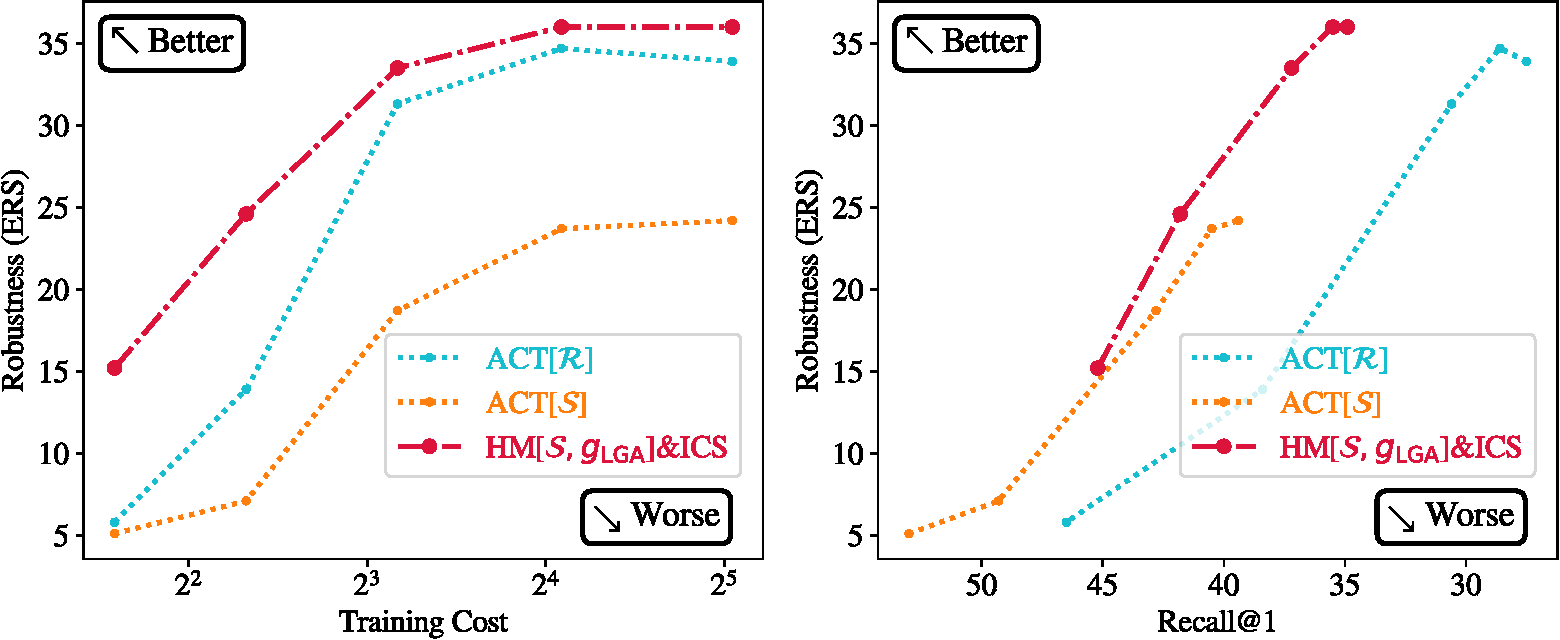
\includegraphics[width=1.0\columnwidth]{introplot.pdf}
	%\vspace{-2.0em}
	\caption{
		%
		Comparison in robustness, training cost, and recall@1 
		between our method (\ie, ``HM[$\mathcal{S},g_\mathsf{LGA}$]\&ICS'')
		and the state-of-the-art method (\ie, ``ACT[$\mathcal{R}$]'' and
		``ACT[$\mathcal{S}$]'') on the CUB Dataset.
		%
	}
	\label{fig:introplot}
\end{figure}

% existing methods & problem

Existing defense methods~\cite{advrank,robrank} are adversarial training-based,
inspired by Madry's \emph{min-max} adversarial training~\cite{madry} because it
is consistently one of the most effective methods for classification task.
%
Specifically, Madry's method involves a inner problem to \emph{maximize} the
loss by perturbing the inputs into adversarial examples, and an outer problem
to \emph{minimize} the loss by updating the model parameters.
%
However, in order to avoid model collapse due to excessively hard examples, the
existing DML defenses refrain from directly adopting such min-max paradigm, but
instead replace the inner problem to indirectly increase the loss value to a
certain level, which suffers from low efficiency and weak adversary (and hence
weak robustness).
%
Since training cost is already a serious issue of adversarial training, the
efficiency in gaining higher adversarial robustness under a lower budget is
inevitable and important for DML defense.

% we argue / insight

Inspired by previous works~\cite{advrank,robrank}, we conjecture that an
appropriate adversary for the inner \emph{maximization} problem should
increase the loss to an ``intermediate''
point between that of benign examples (\ie, unperturbed examples) and the
theoretical upper bound.
%
Such point should be reached by an efficient adversary directly.
%
Besides, we speculate the triplet sampling strategy has a key impact in
adversarial training, because it is also able to greatly influence the
mathematical expectation of loss even without adversarial attack.

% hardness manipulation

In this paper, we first define the ``\emph{hardness}'' of a sample triplet as
the difference between the anchor-positive distance and anchor-negative
distance.
%
Then, Hardness Manipulation (HM) is proposed to adversarially perturb a given
sample triplet and increase its hardness into a specified \emph{destination}
hardness level for adversarial training.
%
The objective of HM is to minimize the L-$2$ norm of the thresholded difference
between the hardness of the given sample triplet and the specified
\emph{destination} hardness.
%
HM is flexible as regular training and min-max adversarial training~\cite{madry}
can be expressed as its boundary cases, as shown in \cref{fig:hmflexible}.
%
Mathematically, when the HM objective is optimized using Projected Gradient
Descent~\cite{madry}, the sign of its gradient with respect to the adversarial
perturbation is the same as that of directly \emph{maximizing} the loss.
%
Thus, the optimization of HM objective can be interpreted as a direct and
efficient \emph{maximization} process of the loss which stops halfway at the
specified \emph{destination} hardness level, \ie, the aforementioned ``intermediate'' point.

% how hard? benign destination

Then, how hard should such ``\emph{destination} hardness'' be?
%
Recall that the model is already prone to collapse with excessively hard benign
triplets~\cite{facenet}, let alone adversarial examples.
%
Thus, intuitively, the \emph{destination} hardness can be the hardness of
another benign triplet which is moderately harder than the given triplet (\eg,
a Semihard~\cite{facenet} triplet).
%
However, in the late phase of training, the expectation of the difference
between such \emph{destination} hardness and that of the given triplet will be
small, leading to weak adversarial examples and inefficient adversarial
learning.
%
Besides, strong adversarial examples in the early phase of training may also
hinder the model from learning good embeddings, and hence influence the
performance on benign examples.
%
In particular, a better \emph{destination} hardness should be able to balance the
training objectives in the early and late phases of training.

% Gradual Adversary

To this end, Graduate Adversary, a family of pseudo-hardness functions is
proposed, which can be used as the \emph{destination} hardness.
%
A function that leads to relatively weak and relatively strong adversarial
examples, respectively in the early and late phase of training belongs to this
family.
%
As an example, we design a ``Linear Graduate Adversary'' (LGA)
function as the linearly scaled negative triplet margin, incorporating a strong
prior that the \emph{destination} hardness should remain Semihard
based on our empirical observation.

% Intra-Class Structure

Additionally, it is noted that a sample triplet will be augmented into a
sextuplet (both benign and adversarial examples) during adversarial training.
%
In this case, the \emph{intra-class} structure can be enforced, which has been
neglected by existing methods.
%
Since some existing attacks aim to change the sample rankings in the same
class~\cite{advrank},
%
we propose a simple \emph{intra-class} structure loss term for adversarial
training, which is expected to further improve adversarial robustness.

% evaluation and conclusion
Comprehensive experiments are conducted on three commonly used DML datasets,
namely CUB-200-2011~\cite{cub200}, Cars-196~\cite{cars196}, and Stanford Online
Product~\cite{sop}.
%
The proposed method overwhelmingly outperforms the state-of-the-art defense in
terms of robustness, training efficiency, as well as the performance on benign
examples.

\begin{figure}
	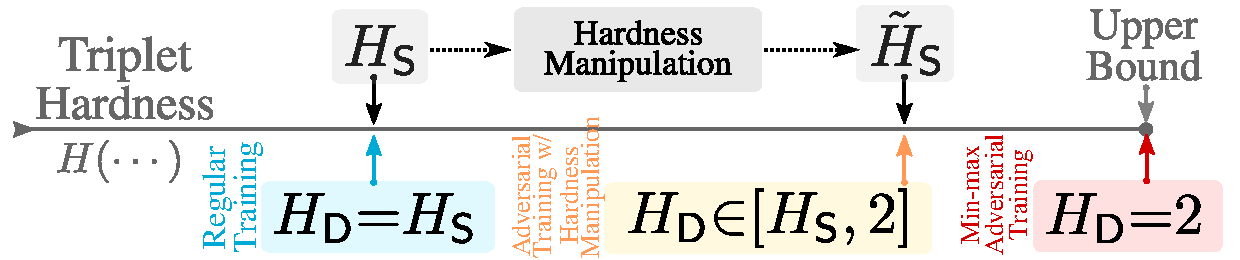
\includegraphics[width=\columnwidth]{hmflexible.pdf}
	\vspace{-1.8em}
	\caption{Flexibility of hardness manipulation.
	%
	Regular training and min-max adversarial training are its boundary cases.
	}
	\label{fig:hmflexible}
\end{figure}

% contributions
In summary, our contributions include proposing:
%
\begin{enumerate}[nosep, noitemsep, leftmargin=*]
	%
	\item {\textit{Hardness Manipulation}} (HM) as a flexible and efficient
		tool to create adversarial example triplets for subsequent adversarial
		training of a DML model.
		%
	\item \textit{Linear Gradual Adversary} (LGA) as a Graduate Adversary, \ie,
		a pseudo-hardness function for HM, which incorporates our empirical
		observations and can balance the training objectives during the
		training process.
		%
	\item \textit{Intra-Class Structure} (ICS) loss term to further improve
		model robustness and adversarial training efficiency, while such structure is
		neglected by existing defenses. 
		%
\end{enumerate}

\section{Related Works}
\label{sec:2}

\begin{comment}
\oo{In potential of future works}
Deep metric learning on adversarial example is also used for improving
adversarial robustness for deep classifiers~\cite{mao2019metric}.
\end{comment}

\textbf{Adversarial Attack.}
%
Szegedy \etal~\cite{l-bfgs} find misclassification of DNN can be triggered by
an imperceptible adversarial perturbation to the input image.
%
Ian \etal~\cite{fgsm} attribute the reason to DNN being locally linear with
respect to the adversarial perturbation.
%
Subsequent first-order gradient-based methods can compromise the DNNs more
effectively under the white-box assumption~\cite{i-fgsm,madry,apgd,lafeat}.
%
In contrast, black-box attacks have been explored by query-based
methods~\cite{nes-atk,spsa-atk} and transferability-based
methods~\cite{di-fgsm}, which are more practical for real-world scenarios.

\textbf{Adversarial Defense.}
%
Various defenses are proposed to counter the attacks.
%
However, defenses incurring gradient masking
lead to a false sense of robustness~\cite{obfuscated}.
%
Defensive distillation~\cite{distill2} is compromised in~\cite{cw}.
%
Ensemble of weak defenses is not
robust~\cite{ensembleweak}.
%
Other defenses such as input
preprocessing~\cite{deflecting}, or randomization~\cite{self-ensemble} are proposed.
%
But many of them are still susceptible to adaptive attacks~\cite{adaptive}.
%
Of all defenses, adversarial training~\cite{madry} consistently remains to be one of the
most effective
methods~\cite{bilateral,advtrain-triplet,benchmarking,smoothat,trades,robustwrn,weightperturb,featurescatter},
but suffers from high training cost~\cite{freeat,fastat,yopo}, performance drop on
benign examples~\cite{odds,geometry,onmanifold}, and overfitting on adversarial examples~\cite{bagoftricks,overfitting}.

\textbf{Deep Metric Learning.}
%
A wide range of applications such as image retrieval~\cite{imagesim2},
cross-modal retrieval~\cite{ladderloss}, and face recognition~\cite{facenet}
can be formulated as a DML problem.
%
A well-designed loss function and a proper sampling method are crucial for DML
performance~\cite{dmlreality}.  For instance, the classical
triplet loss~\cite{facenet} could reach state-of-the-art performance with an appropriate
sampling strategy~\cite{revisiting}.

\textbf{Attacks in DML.}
%
DML has been found vulnerable to adversarial attacks as
well~\cite{advrank,advorder,robrank}, which raises concerns on safety,
security, or fairness for a DML application.
%
The existing attacks aim to completely subvert the image retrieval
results~\cite{qair,learn-to-misrank,advdpqn,advpattern,flowertower,universalret},
or covertly alter the top-ranking results without being
abnormal~\cite{advrank,advorder}.

%
\textbf{Defenses in DML.} Unlike attacks, defenses are less explored.
%
Embedding Shifted Triplet (EST)~\cite{advrank} is an
adversarial training method using adversarial examples with maximized embedding
move distance off their original locations.
%
The state-of-the-art method, \ie,
Anti-Collapse Triplet (ACT)~\cite{robrank} forces the model to separate
collapsed positive and negative samples apart in order to learn robust
features.
%
However, both EST and ACT suffer from low efficiency as the
inner problem is replaced into an indirect adversary.

\section{Our Approach}
\label{sec:3}

% Background DML formulation

In DML~\cite{revisiting,dmlreality}, a 
function $\phi:\mathcal{X}{\mapsto}\Phi \subseteq \mathbb{R}^D$ is learned to
map data points $\mX\in\mathcal{X}$ into an embedding space $\Phi$, which is usually
normalized to the real unit hypersphere for regularization.
%
With a predefined distance function $d(\cdot,\cdot)$, which is usually the
Euclidean distance, we can measure the distance between $\mX_i$ and $\mX_j$ as
$d_\phi(\mX_i,\mX_j)=d(\phi(\mX_i),\phi(\mX_j))$.
%
Typically, the triplet loss~\cite{facenet} can be used to learn the
embedding function, and it could reach the state-of-the-art performance with an
appropriate triplet sampling strategy~\cite{revisiting}.

% Background Triplet loss

Given a triplet of anchor, positive, negative images, \ie, $\mA, \mP,
\mN \in \mathcal{X}$, we can calculate their embeddings with $\phi(\cdot)$ as
$\va, \vp, \vn$, respectively.
%
Then triplet loss~\cite{facenet} is defined as:
%\setlength{\belowdisplayskip}{0pt} \setlength{\belowdisplayshortskip}{0pt}
%\setlength{\abovedisplayskip}{0pt} \setlength{\abovedisplayshortskip}{0pt}
%
\begin{equation}
%
	L_\text{T}(\va, \vp, \vn; \gamma) = \max(0, d(\va, \vp) - d(\va, \vn) +
	\gamma),
	\end{equation}
%
%$
%
where $\gamma$ is a predefined margin parameter.
%
To attack the DML model, an imperceptible adversarial perturbation $\vr \in
\Gamma$ is added to the input image $\mX$, where $\Gamma = \{\vr | \mX+\vr\in
\mathcal{X},  \|\vr\|_p \leq \varepsilon\}$, so that its embedding vector
$\tilde{\vx}=\phi(\mX+\vr)$ will be moved off its original location towards
other positions to achieve the attacker's goal.
%
To defend against the attacks, the DML model can be adversarially trained to
reduce the effect of attacks~\cite{advrank,robrank}.
%
The most important metrics for a good defense are adversarial
robustness, training efficiency, and performance on benign examples.

\subsection{Hardness Manipulation}
\label{sec:31}

% define hardness

Given an image triplet ($\mA$, $\mP$, $\mN$) sampled with a certain sampling
strategy (\eg, Random) within a mini-batch, we define its ``\emph{hardness}''
as a scalar which is within $[-2,2]$:
%
\begin{equation}
%
H(\mA,\mP,\mN)=d_\phi(\mA,\mP)-d_\phi(\mA,\mN).
%
\end{equation}
%
Clearly, it is an internal part of the triplet loss.
%
For convenience, we call this triplet ($\mA$, $\mP$, $\mN$) as ``\emph{source}
triplet'', and its corresponding hardness value as ``\emph{source} hardness'',
denoted as $H_\mathsf{S}$.

% define hardness manipulation

Then, \emph{Hardness Manipulation} (HM) aims to increase the \emph{source}
hardness $H_\mathsf{S}$ into a specified ``\emph{destination} hardness''
$H_\mathsf{D}$, by finding adversarial examples of the source triplet, \ie,
$(\mA{+} {\vr}_a, \mP {+} {\vr}_p, \mN {+} {\vr}_n)$, where $({\vr}_a, {\vr}_p,
{\vr}_n)$ are the adversarial perturbations.
%
Denoting the hardness of the adversarially perturbed \emph{source} triplet
as $\tilde{H}_\mathsf{S}$, \ie,
%
$\tilde{H}_\mathsf{S} = H(\mA{+} {\vr}_a, \mP {+} {\vr}_p, \mN {+} {\vr}_n)$,
%
the HM is implemented as:
%
\begin{equation}
	%
	\hat{\vr}_a, \hat{\vr}_p, \hat{\vr}_n = \argmin_{\vr_a,\vr_p,\vr_n}
	\big\|\max(0, H_\mathsf{D} - \tilde{H}_\mathsf{S} ) \big\|_2^2.
	%
	\label{eq:hm}
	%
\end{equation}
%
The $\max(0,\cdot)$ part in \cref{eq:hm} truncates the gradient when
$\tilde{H}_\mathsf{S}>H_\mathsf{D}$, automatically stopping the optimization, because
$\tilde{H}_\mathsf{S}$ is not desired to be reduced once it exceeds $H_\mathsf{D}$.
%
 \cref{eq:hm} is written in the L-$2$ norm form instead of the standard Mean
Squared Error because HM can be directly extended into vector form for a
mini-batch.
%
The optimization problem can be solved by Projected Gradient Descent
(PGD)~\cite{madry}.
%
And the resulting adversarial examples are used for adversarially training the
DML model with
%
$L_\text{T}(\phi(\mA+\hat{\vr}_a), \phi(\mP+\hat{\vr}_p),
\phi(\mN+\hat{\vr}_n))$.
%
The overall procedure of HM is illustrated in \cref{fig:hm}.
%
For convenience,
we abbreviate the adversarial training with adversarial examples created
through this way as ``$\text{HM}[H_\mathsf{S},H_\mathsf{D}]$'' in this paper.

\begin{figure}
	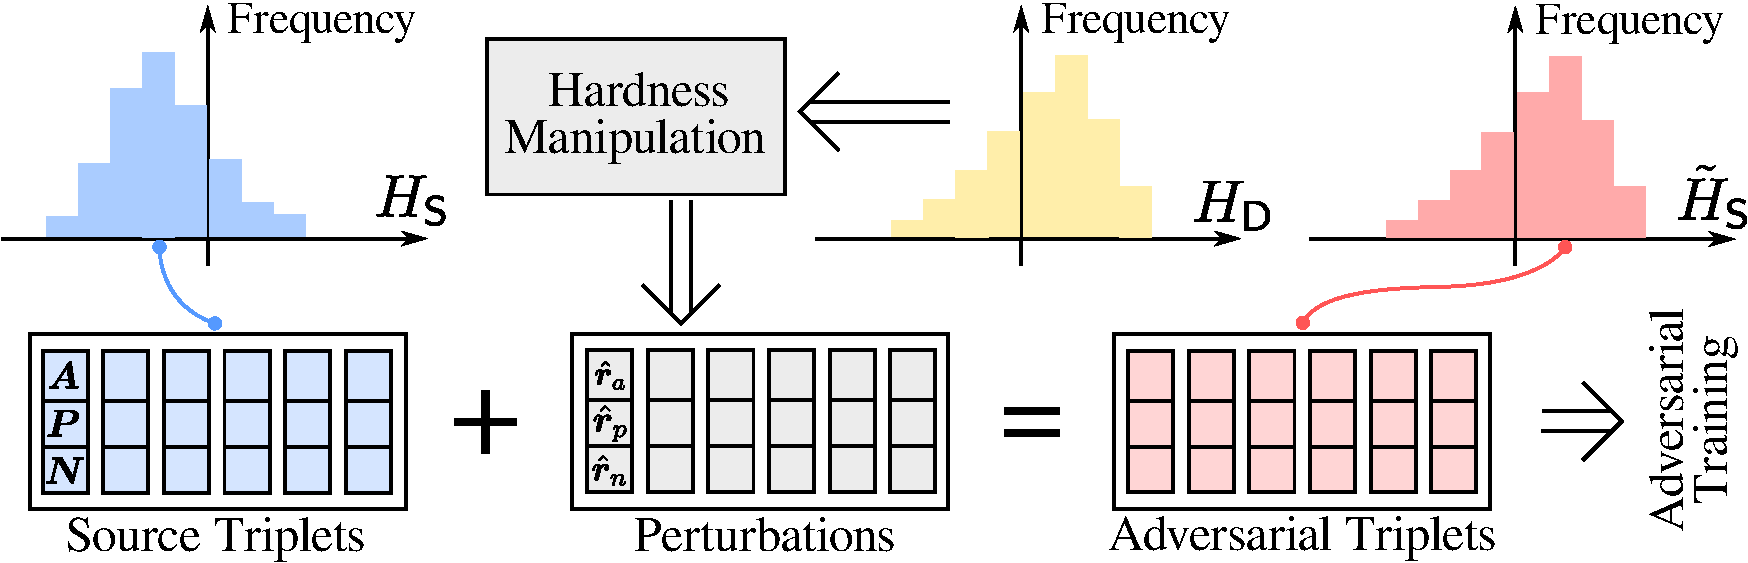
\includegraphics[width=\columnwidth]{hmillust.pdf}
	\vspace{-1.8em}
	\caption{Illustration of hardness manipulation.}
	\label{fig:hm}
\end{figure}

% strong adversary

Note, in the PGD case, the sign of negative gradient of the HM objective
\emph{w.r.t.} an adversarial perturbation $\vr$ is equivalent to the sign of
gradient for directly maximizing $\tilde{H}_\mathsf{S}$ (hence
maximizing $L_\text{T}$) when $H_\mathsf{D}>\tilde{H}_\mathsf{S}$, \ie,
%
\begin{align}
	\Delta \vr
	=&
	\sign\big\{
		-\frac{\partial}{\partial \vr} \big\| \max(0, 
		H_\mathsf{D} - \tilde{H}_\mathsf{S} ) \big\|_2^2
	\big\}
	\\
	=&
	\sign\big\{
		2(H_\mathsf{D} - \tilde{H}_\mathsf{S})
		\frac{\partial }{\partial \vr} \tilde{H}_\mathsf{S} \big\}
	=
	\sign\big\{
		\frac{\partial}{\partial \vr} \tilde{H}_\mathsf{S}
		\big\}.
\end{align}
%
The perturbation $\vr$ is updated as $\vr \leftarrow \text{Proj}_\Gamma\{\vr + \alpha \Delta
\vr\}$ by PGD for $\eta$ steps with a step size $\alpha$, where the ``Proj'' operator
clips the result into the $\Gamma$ set.
%
Thus, the optimization of HM objective can be interpreted as direct
maximization of $\tilde{H}_\mathsf{S}$, which discontinues very early once it
exceeds $H_\mathsf{D}$.
%
With HM, the model can learn from an \emph{efficient} adversary.

Since the same $\Delta\vr$ can be used for both minimizing the HM objective
and maximizing the triplet loss, one potential advantage of HM is that
the gradients during the training process can be reused for creating
adversarial examples for much faster adversarial training, according to 
Free Adversarial Training~\cite{freeat}.
%
We leave this for future exploration.

% selection of destination hardness

\textbf{Destination Hardness}.
%
$\text{HM}[H_\mathsf{S},H_\mathsf{D}]$ is flexible as various
types of $H_\mathsf{D}$ can be specified, \eg, a constant, the
hardness of another benign triplet, or a pseudo-hardness function.
%
The case of maximizing the triplet loss is equivalent to
$\text{HM}[H_\mathsf{S},2]$, where $2$ is the 
upper bound of hardness, while $\text{HM}[H_\mathsf{S},H_\mathsf{S}]$
is regular DML training, as shown in \cref{fig:hmflexible}.

As pushing $\tilde{H}_\mathsf{S}$ towards the upper bound will easily render
model collapse, a valid $H_\mathsf{D}$ should be chosen within the interval
$[H_\mathsf{S},2]$.
%
Thus, intuitively, $H_\mathsf{D}$ can be the hardness of another benign triplet
(with the same anchor) sampled with a strategy with a higher hardness
expectation, \ie, $E[H_\mathsf{D}] > E[H_\mathsf{S}]$.
%
Or at least the $\text{Var}[H_\mathsf{D}]$ of another benign triplet has to
be large enough (for a small portion of triplets $H_\mathsf{D}>H_\mathsf{S}$)
in order to create a notable number of valid adversarial
examples.
%
For instance, $H_\mathsf{D}$ can be the hardness of a Semihard~\cite{facenet}
triplet when the \emph{source} triplet is sampled with Random sampler.
%
Predictably, the model performance will be significantly influenced by the
triplet sampling strategies we chose for $H_\mathsf{D}$ in this case.
%
For convenience of further discussion, we denote the hardness of a Random,
Semihard, and Softhard triplets as $\mathcal{R}$, $\mathcal{M}$, $\mathcal{S}$,
respectively.

If we have a strong prior knowledge on what the \emph{destination} hardness
should be, then we can even use a pseudo-hardness function $g(\cdot)$, \ie, a
customized scalar function.



\subsection{Gradual Adversary}
\label{sec:32}

\begin{figure}
	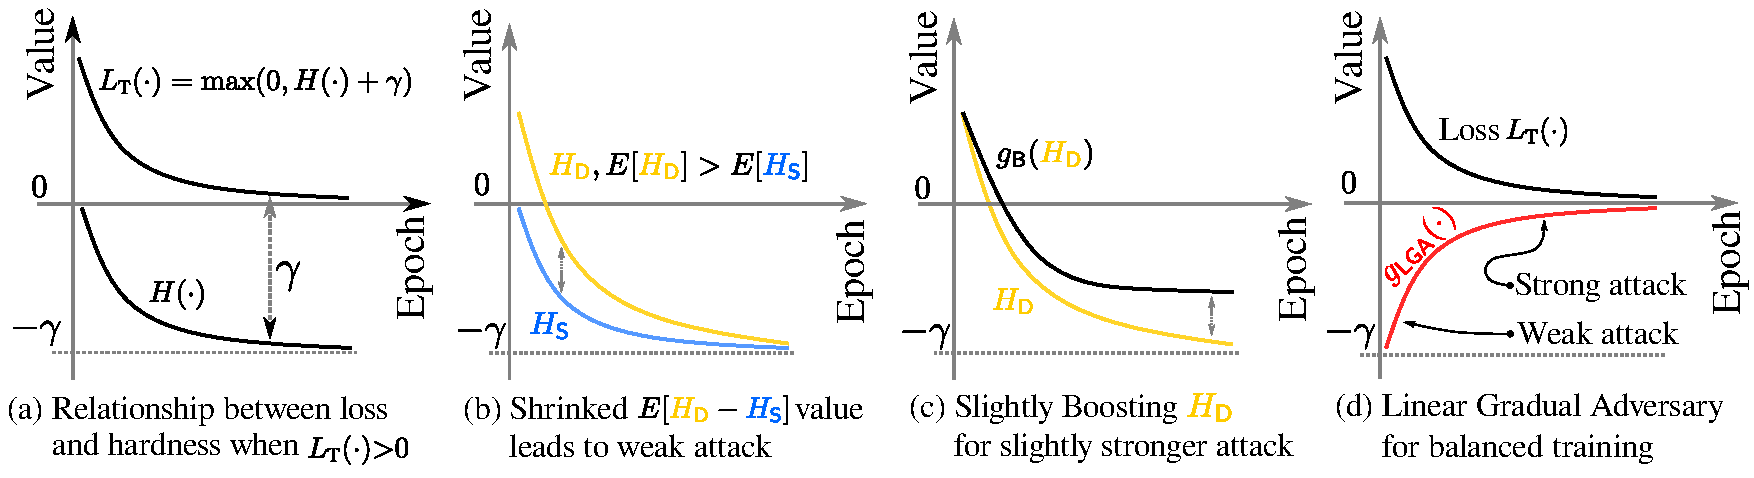
\includegraphics[width=\columnwidth]{gaillust.pdf}
	\caption{Illustration of (linear) gradual adversary.}
	\label{fig:ga}
\end{figure}


% motivation of GA : late phase

Even if $H_\mathsf{D}$ is calculated from another triplet harder than the
\emph{source} triplet, the adversarial example may become weak in the late
phase of training.
%
The optimizer aims to reduce the expectation of 
loss $E[L_\text{T}]$ towards zero as possible over the distribution of triplets, and thus
the $E[H]$ of any given triplet will tend to $-\gamma$, reducing the
hardness of adversarial triplets from HM as $E[H_\mathsf{D}-H_\mathsf{S}]$
decreases accordingly.
%
Weakened adversarial examples are insufficient for robustness.

% hardness boosting

Intuitively, such deficiency can be alleviated with a \emph{pseudo-hardness}
function that slightly increases the value of $H_\mathsf{D}$ in the late phase
of training.
%
Denoting the loss value from the previous training iteration as $\ell_{t-1}$,
we first normalize it into $[0,1]$ as $\bar{\ell}_{t-1}=\min(u,\ell_{t-1})/u$,
where $u$ is a manually specified constant.
%
Then we can linearly shift the $E[H_\mathsf{D}]$ by a scaled constant $\xi$,
\ie,
%
\begin{equation}
	%
	g_\mathsf{B}(H_\mathsf{D};\xi,\bar{\ell}_{t-1}) =
	H_\mathsf{D} + \xi \cdot (1-\bar{\ell}_{t-1}).
	%
\end{equation}
%
The deficiency can be alleviated in
$\text{HM}[H_\mathsf{S},g_\mathsf{B}(H_\mathsf{D})]$.


% motivation of GA: early phase

Apart from the deficiency in the late phase of training, we speculate that
relatively strong adversarial examples may hinder the model from 
learning good embedding space for the benign examples in the very early phase
of training, hence influence the model performance on benign examples.

% Gradual Adversary

Thus, $H_\mathsf{D}$ should lead to (1) relatively weak adversarial examples in
the early training phase (indicated by a large loss value), and (2) relatively
strong adversarial examples in the late training phase (indicated by a small
loss value),
%
in order to automatically balance the training objectives (\ie, performance on
benign examples \emph{v.s.} robustness).
%
A satisfactory pseudo-hardness function is a ``Graduate Adversary''.

% Linear graduate adversary

As an example, we propose a ``Linear Gradual Adversary'' (LGA) pseudo-hardness
function that is independent to any benign triplets, incorporating our empirical
observation that $H_\mathsf{D}$ should remain Semihard~\cite{facenet}, as
follows:
%
\begin{equation}
	%
	g_\mathsf{LGA}(\bar{\ell}_{t-1}) = -\gamma \cdot \bar{\ell}_{t-1} ~ \in
	[-\gamma,0].
	%
\end{equation}
%
Our empirical observation is obtained from \cref{sec:41}.
%
And the training objectives, namely performance on benign examples and
robustness will be automatically balanced in
$\text{HM}[H_\mathsf{S},g_\mathsf{LGA}]$, leading to a better eventual overall
performance, as illustrated in \cref{fig:ga}.
%
More complicated or non-linear pseudo-hardness functions are left for future study.
%for sake of simplicity.
%

\subsection{Intra-Class Structure}
\label{sec:33}

\begin{figure}[t]
	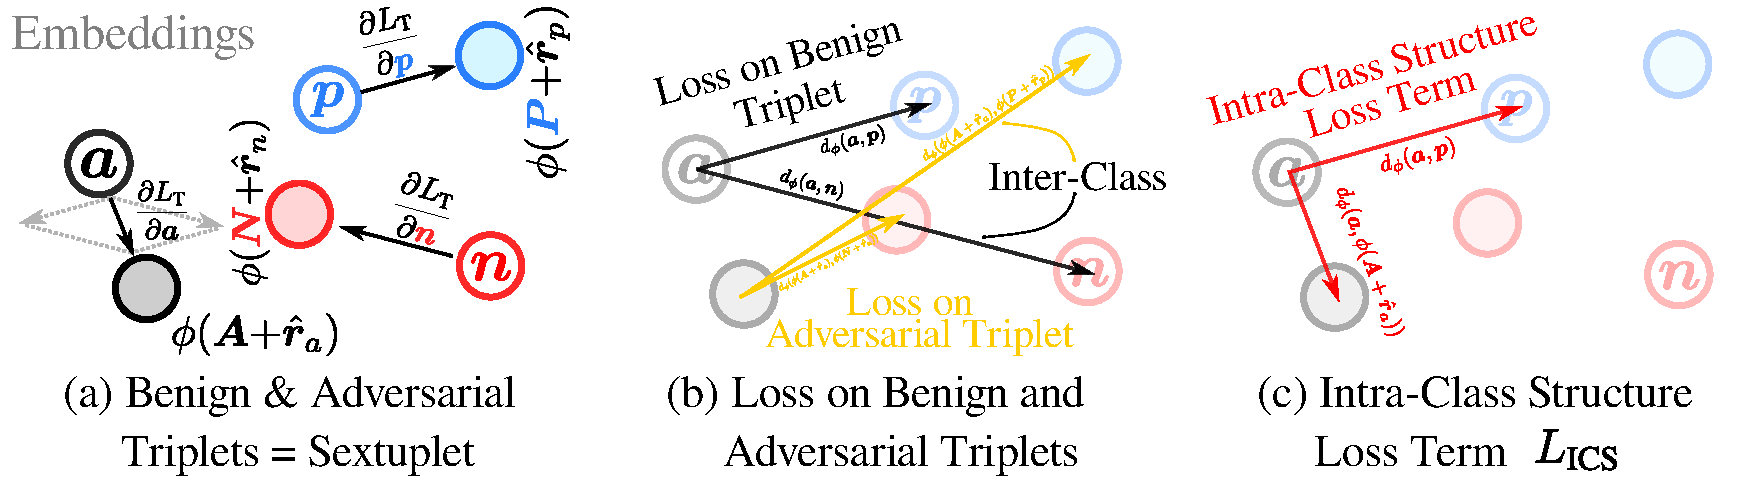
\includegraphics[width=1.0\columnwidth]{icsapn.pdf}
	\caption{Illustration of intra-class structure loss term.}
	\label{fig:ics}
\end{figure}

% motivation

During adversarial training with HM, the adversarial counterpart of each given sample
triplet is fed to the model, and the triplet loss will enforce a good
\emph{inter-class} structure.
%
Since the anchor, positive sample, and their adversarial counterpart belongs to
the same class, it should be noted that the \emph{intra-class} structure can be
enforced as well, but this has been neglected by the existing DML defenses.
%
\emph{Intra-class} structure is also important for robustness besides the
\emph{inter-class} structure, because the attack may attempt to change the
rankings of samples in the same class~\cite{advrank}.

% Solution

We propose an additional loss function term to enforce such \emph{intra-class}
structure, as shown in \cref{fig:ics}.
%
Specifically, the anchor $\va$ and its adversarial counterpart
are separated from the positive sample $\vp$ by reusing the triplet loss,
\ie,
%
\begin{equation}
	L_\text{ICS} = \lambda \cdot L_\text{T}(
	\va, \phi(\mA + \hat{\vr}_a), \vp; 0),
\end{equation}
%
where $\lambda$ is a constant weight for this loss term,
and the margin is set as zero to avoid negative effect.
%
The $L_\text{ICS}$ term can be appended to the loss function for
adversarial training.

\section{Experiments}
\label{sec:4}

% evaluation: dataset

To validate our defense method, we conduct experiments
on three commonly used DML datasets: CUB-200-2011 (CUB)~\cite{cub200}, Cars-196
(CARS)~\cite{cars196}, and Stanford-Online-Product (SOP)~\cite{sop}.
%
We follow the same experimental setup as that used in the state-of-the-art
defense work~\cite{robrank} and standard DML~\cite{revisiting} for ease of comparison.

\begin{table}
\resizebox{\columnwidth}{!}{
	\setlength{\tabcolsep}{0.8em}
\begin{tabular}{c|ccccc}
\toprule
Statistics & Random & Semihard & Softhard & Distance & Hardest\tabularnewline
\midrule
$E[H]$ & $-0.164$ & $-0.126$ & $-0.085$ & $0.043$ & $0.044$\tabularnewline
$\text{Var}[H]$ & $0.00035$ & $0.00013$ & $0.00122$ & $0.00021$ & $0.00021$\tabularnewline
\bottomrule
\end{tabular}
}

	\caption{Mean \& Variance of Hardness w/ Various Triplet Samplers.
	}

	\label{tab:hsort}
\end{table}


% evaluation: configuration

Specifically, we (adversarially) train ImageNet-initialized ResNet-18
(RN18)~\cite{resnet} with the output dimension of the last layer changed to
$N{=}512$.
%
The margin $\gamma$ in the triplet loss is $0.2$.
%
Adam~\cite{adam} optimizer is used for parameter updates, with a learning rate
of $1.0{\times}10^{-3}$ for $150$ epochs, and a mini-batch size of $112$.
%
Adversarial examples are created within $\Gamma$ with
$\varepsilon{=}8/255$ and $p{=}\infty$, using PGD~\cite{madry} with step size
$\alpha{=}1/255$ and a default maximum step number $\eta{=}8$.
%
The parameter $u$ is equal to $\gamma$, much less than the loss upper bound
in order to avoid excessive hardness boost in $g_\mathsf{B}$ and $g_\mathsf{LGA}$.
%
Parameter $\lambda$ for $L_\text{ICS}$ is $0.5$ by default ($0.05$ on SOP).

The model performance on the benign (\ie, unperturbed) examples is measured in terms of 
Recall@1 (R@1), Recall@2 (R@2), mAP and NMI
following~\cite{revisiting,robrank}.
%
The adversarial robustness of a model is measured in Empirical Robustness Score
(ERS)~\cite{robrank}, a normalized score (the higher the better) from
a collection of (simplified white-box) attacks against DML, which are
optimized with PGD ($\eta=32$ for strong attack).
%
Since adversarial training is not ``gradient masking''~\cite{obfuscated}, the
performance of white-box attack can be regarded as the upper bound of the
black-box attacks, and thus a model that is empirically robust to the collection
of white-box attacks is expected to be robust in general.

Concretely, the collection of attacks for ERS include:
%
(1) CA+, CA-, QA+ and QA-~\cite{advrank}, which move some selected candidates
towards the topmost or bottommost part of ranking list;
%
(2) TMA~\cite{flowertower} which increases the cosine similarity between two arbitrary samples;
%
(3) ES~\cite{advrank,advdpqn}, which moves the embedding of a sample off its original position as
distant as possible;
%
(4) LTM~\cite{learn-to-misrank}, which perturbs the ranking result by minimizing the distance of
unmatched pairs while maximizing the distance of matched pairs;
%
(5) GTM~\cite{robrank}, which minimizes the distance between query and the
closest unmatching sample.
%
(6) GTT~\cite{robrank}, aims to move the top-$1$ candidate out of the top-$4$
retrieval results, which is simplified from \cite{qair}.
%
The setup of all the attacks for robustness evaluation are unchanged from
\cite{robrank} for fair comparison.
%
Further details of these attacks can be found in \cite{robrank}.

\subsection{Selection of Source \& Destination Hardness}
\label{sec:41}

\begin{table}
\resizebox{\columnwidth}{!}{
\setlength{\tabcolsep}{0.36em}
\begin{tabular}{c|cc|cc|cc|cc|cc}
	\toprule

	\multirow{2}{*}{\backslashbox{$H_\mathsf{S}$}{$H_\mathsf{D}$}} & \multicolumn{2}{c|}{Random} & \multicolumn{2}{c|}{Semihard} & \multicolumn{2}{c|}{Softhard} & \multicolumn{2}{c|}{Distance} & \multicolumn{2}{c}{Hardest}\tabularnewline
\cline{2-11} \cline{3-11} \cline{4-11} \cline{5-11} \cline{6-11} \cline{7-11} \cline{8-11} \cline{9-11} \cline{10-11} \cline{11-11} 
& R@1 & ERS & R@1 & ERS & R@1 & ERS & R@1 & ERS & R@1 & ERS\tabularnewline

\midrule

Random & \cellcolor{black!10}53.9 & \cellcolor{black!10}3.8 & 27.0 & 35.1 & \multicolumn{2}{c|}{Collapse} & \multicolumn{2}{c|}{Collapse} & \multicolumn{2}{c}{Collapse}\tabularnewline
\hline
Semihard & 43.9 & 5.4 & \cellcolor{black!10}44.0 & \cellcolor{black!10}5.0 & \multicolumn{2}{c|}{Collapse} & \multicolumn{2}{c|}{Collapse} & \multicolumn{2}{c}{Collapse}\tabularnewline
\hline
Softhard & 48.3 & 13.7 & 38.4 & 29.6 & \cellcolor{black!10}55.7 & \cellcolor{black!10}6.2 & \multicolumn{2}{c|}{Collapse} & \multicolumn{2}{c}{Collapse}\tabularnewline
\hline
Distance & 52.7 & 4.8 & 50.7 & 4.8 & \multicolumn{2}{c|}{Collapse} & \cellcolor{black!10}51.4 & \cellcolor{black!10}4.9 & 54.7 & 5.4\tabularnewline
\hline
Hardest & 51.0 & 4.7 & 52.2 & 4.8 & \multicolumn{2}{c|}{Collapse} & 52.6 & 5.1 & \cellcolor{black!10}48.9 & \cellcolor{black!10}5.0\tabularnewline

	\bottomrule
\end{tabular}
}

	\caption{Combinations of Source \& Destination Hardness.
	%
	Evaluated on CUB Dataset with RN18 model.
	%
	The last-epoch performance is reported instead of the peak performance.
	%
	Models on the diagonal are regularly (instead of adversarially) trained.
	%
}
	\label{tab:desth}

\end{table}


\begin{table*}
\resizebox{\linewidth}{!}{
	\setlength{\tabcolsep}{0.2em}




\begin{tabular}{cc|cccc|ccccc|ccccc|c}
\hline 
\multicolumn{1}{c|}{\multirow{2}{*}{\textbf{Dataset}}} & \multirow{2}{*}{\textbf{Defense}} & \multicolumn{4}{c|}{\textbf{Benign Example}} & \multicolumn{10}{c|}{\textbf{White-Box Attacks for Robustness Evaluation}} & \multirow{2}{*}{\textbf{ERS$\uparrow$}}\tabularnewline
\cline{3-16} \cline{4-16} \cline{5-16} \cline{6-16} \cline{7-16} \cline{8-16} \cline{9-16} \cline{10-16} \cline{11-16} \cline{12-16} \cline{13-16} \cline{14-16} \cline{15-16} \cline{16-16} 
 &  & R@1$\uparrow$ & R@2$\uparrow$ & mAP$\uparrow$ & NMI$\uparrow$ & CA+$\uparrow$ & CA-$\downarrow$ & QA+$\uparrow$ & QA-$\downarrow$ & TMA$\downarrow$ & ES:D$\downarrow$ & ES:R$\uparrow$ & LTM$\uparrow$ & GTM$\uparrow$ & GTT$\uparrow$ & \tabularnewline
\hline 
\hline 
CUB & N/A & 53.9 & 66.4 & 26.1 & 59.5 & 0.0 & 100.0 & 0.0 & 99.9 & 0.883 & 1.762 & 0.0 & 0.0 & 14.1 & 0.0 & 3.8\tabularnewline
\hline 
 & ACT ($\eta=2$) & 46.5 & 58.4 & 29.1 & 55.6 & 0.6 & 98.9 & 0.4 & 98.1 & 0.837 & 1.666 & 0.2 & 0.2 & 19.6 & 0.0 & 5.8\tabularnewline
 & ACT ($\eta=4$) & 38.4 & 49.8 & 22.8 & 49.7 & 4.6 & 81.9 & 2.8 & 80.5 & 0.695 & 1.366 & 2.9 & 2.3 & 18.8 & 0.1 & 13.9\tabularnewline
 & ACT ($\eta=8$) & 30.6 & 40.1 & 16.5 & 45.6 & 13.7 & 46.8 & 12.6 & 39.3 & 0.547 & 0.902 & 13.6 & 9.8 & 21.9 & 1.3 & 31.3\tabularnewline
 & ACT ($\eta=16$) & \uline{28.6} & \uline{38.7} & \uline{15.1} & \uline{43.7} & \uline{15.8} & \uline{37.9} & \uline{16.0} & \uline{31.5} & \uline{0.496} & \uline{0.834} & \uline{11.3} & \uline{9.8} & \uline{21.2} & \uline{2.1} & \uline{34.7}\tabularnewline
v7 & ACT ($\eta=16$) & R:V &  &  &  &  &  &  &  &  &  &  &  &  &  & \tabularnewline
 & ACT ($\eta=32$) & 27.5 & 38.2 & 12.2 & 43.0 & 15.5 & 37.7 & 15.1 & 32.2 & 0.472 & 0.821 & 11.1 & 9.4 & 14.9 & 1.0 & 33.9\tabularnewline
\hline 
 & HM{[}$\mathcal{R},\mathcal{M}${]} ($\eta=2$) & 34.3 & 44.9 & 19.5 & 47.4 & 7.7 & 77.5 & 6.5 & 70.8 & 0.636 & 1.281 & 4.3 & 2.6 & 21.1 & 0.2 & 18.1\tabularnewline
 & HM$|_{\text{Random}}^{\text{Semihard}}$ ($\eta=4$) & 30.7 & 40.3 & 16.4 & 45.3 & 13.9 & 60.4 & 13.5 & 48.1 & 0.582 & 1.041 & 6.6 & 6.6 & 20.2 & 1.2 & 27.1\tabularnewline
 & HM$|_{\text{Random}}^{\text{Semihard}}$ ($\eta=8$) & 27.0 & 36.0 & 13.2 & 42.5 & 19.4 & 48.0 & 22.2 & 32.0 & 0.535 & 0.867 & 11.6 & 10.4 & 19.3 & 2.9 & 35.1\tabularnewline
 & HM$|_{\text{Random}}^{\text{Semihard}}$ ($\eta=16$) & 23.8 & 32.6 & 11.6 & 40.6 & 20.9 & 45.0 & 24.6 & 28.6 & 0.494 & 0.805 & 15.6 & 11.3 & 22.1 & 3.2 & 38.0\tabularnewline
 & HM$|_{\text{Random}}^{\text{Semihard}}$ ($\eta=32$) & 23.1 & 31.9 & 11.3 & 40.3 & 22.8 & 46.0 & 24.3 & 28.3 & 0.495 & 0.800 & 14.2 & 11.7 & 19.7 & 3.8 & 38.0\tabularnewline
\hline 
 & HM$|_{\text{Softhard}}^{\text{Semihard}}$ ($\eta=2$) & 44.5 & 56.1 & 27.8 & 53.3 & 1.9 & 87.7 & 1.6 & 88.8 & 0.827 & 1.101 & 3.7 & 0.3 & 19.0 & 0.0 & 11.6\tabularnewline
 & HM$|_{\text{Softhard}}^{\text{Semihard}}$ ($\eta=4$) & 40.6 & 51.8 & 24.2 & 51.0 & 7.3 & 64.1 & 6.3 & 60.9 & 0.715 & 0.894 & 7.9 & 4.4 & 22.8 & 0.2 & 22.1\tabularnewline
 & HM$|_{\text{Softhard}}^{\text{Semihard}}$ ($\eta=8$) & 38.4 & 49.7 & 22.9 & 50.3 & 10.9 & 50.5 & 10.8 & 44.6 & 0.680 & 0.722 & 13.3 & 11.2 & 25.8 & 1.2 & 29.6\tabularnewline
 & HM$|_{\text{Softhard}}^{\text{Semihard}}$ ($\eta=16$) & 36.0 & 46.2 & 20.6 & 48.5 & 14.5 & 39.7 & 15.8 & 32.8 & 0.587 & 0.678 & 18.6 & 16.8 & 27.6 & 3.1 & 36.2\tabularnewline
 & HM$|_{\text{Softhard}}^{\text{Semihard}}$ ($\eta=32$) & Q &  &  &  &  &  &  &  &  &  &  &  &  &  & \tabularnewline
\end{tabular}

}

\caption{Efficiency of Hardness Manipulation for Adversarial Training.}
\label{tab:hmeff}
\end{table*}


% where to start

As discussed in \cref{sec:31}, we start from the $H_\mathsf{D}$ calculated from
a harder benign triplet sampled by a different strategy, such as Random,
Semihard~\cite{facenet}, Softhard~\cite{revisiting},
Distance-weighted~\cite{distance} (\emph{abbr}., Distance), or the within-batch
Hardest negative sampling strategy, because we know these strategies do not
result in model collapse in regular training.

% combinations

HM is flexible so that any existing or future triplet sampling strategy
can be used for the source triplet or calculating $H_\mathsf{D}$.
%
But not all potential combinations are expected to be effective for HM, as it
will not create an adversarial triplet when $H_\mathsf{S}\geqslant
H_\mathsf{D}$.
%
Thus, we sort the strategies based on the mean hardness of their
outputs in~\cref{tab:hsort}.
%
Then we adversarially train models on the CUB dataset with all combinations
respectively, and summarize their R@1 and ERS in \cref{tab:desth}.


% 3. table: upper and lower

For cases in the upper triangular of \cref{tab:desth} where $E[H_\mathsf{S}]
\leqslant E[H_\mathsf{D}]$, most of the given triplets will be turned
adversarial.
%
Although almost all of them end up with model collapse, the
$\text{HM}[\mathcal{R},\mathcal{M}]$ is still effective in improving the
robustness, with an expected performance drop in R@1.
%
The combination of Distance and Hardest triplets does not trigger model
collapse due to the small $E[H_\mathsf{D}-H_\mathsf{S}]$, which leads to weak
adversarial examples and a negligible robustness gain.

For cases in lower triangular of \cref{tab:desth}, where $E[H_\mathsf{S}]
\geqslant E[H_\mathsf{D}]$, a large portion of given triplets will be unchanged
according to \cref{eq:hm}, and hence lead to weak robustness.
%
As an exception, $\text{HM}[\mathcal{S},\mathcal{M}]$ is still effective in
improving adversarial robustness, where a notable number of adversarial
examples are created due the high $\text{Var}[H]$ of Softhard.
%
Although $E[H]$ of Softhard is less than that of Distance or Hardest, some hard
adversarial examples are still created%
%
\footnote{Differently, Softhard also samples a
hard positive instead of a random positive besides a hard negative.
%
As a result, the hardness of a small number of Softhard triplets will be 
greater than that of a given Hardest triplet.}
%
due to its large $\text{Var}[H]$, which
still result in a slow collapse.

% 4. summary

In practice, HM creates mini-batches mixing some unperturbed source triplets and
some adversarial triplets.
%
The $\text{HM}[\mathcal{R}, \mathcal{M}]$ and $\text{HM}[\mathcal{S},
\mathcal{M}]$ achieve such balanced mixtures.
%
Subsequent experiments will be based on the two effective combinations.
%
Empirically, the hardness range of Semihard strategy,
\ie, $[-\gamma,0]$ is found appropriate for $H_\mathsf{D}$.

\subsection{Effectiveness of Our Approach}
\label{sec:42}


% What we do

\noindent\textbf{I. Hardness Manipulation.}
%
To validate HM with $H_\mathsf{D}$ calculated from benign
triplets, we adversarially train models using $\text{HM}[\mathcal{R},
\mathcal{M}]$ and $\text{HM}[\mathcal{S}, \mathcal{M}]$ on the CUB dataset,
with varying PGD steps, \ie, $\eta\in\{2,4,8,16,32\}$, respectively.
%
The results can be found in \cref{tab:hmeff}.
%
The performance of the state-of-the-art defense, \ie, ACT~\cite{robrank} is
provided as a baseline.
%
ACT[$\mathcal{R}$] and ACT[$\mathcal{S}$] mean the training triplet is sampled
using Random and Softhard strategy, respectively.
%
We also plot curves in \cref{fig:hmeff} based on the robustness, training
cost\footnote{Training cost is the number of times for forward and backward
propagation in each adversarial training iteration, which is calculated as
$\eta+1$.}, as well as the R@1 performance on benign examples.

% first review the sota curve

As shown, ACT[$\mathcal{R}$] can achieve a high ERS, but with a significant
performance drop in R@1, while ACT[$\mathcal{S}$] can retain a relative high
R@1, but is much less efficient in gaining robustness under a fixed training
cost.
%
Notably, ACT relies on the attack that can successfully pull the adversarial
positive and negative samples close to each other in order to learn robust
features~\cite{robrank}.
%
As a result, ACT's ERS with a small $\eta$ (indicating a weak attack effect) is
relatively low.

\begin{figure}[t]
	%
	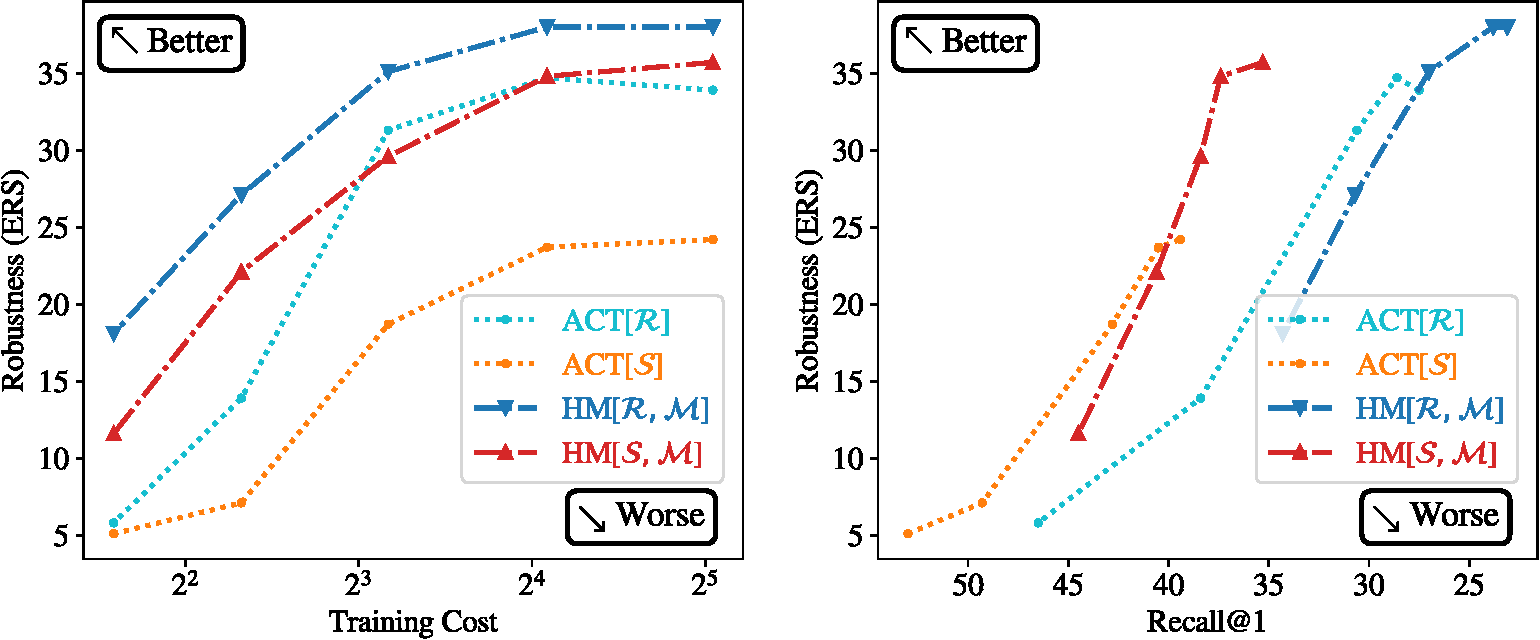
\includegraphics[width=\columnwidth]{fighmeff.pdf}
	%
	\vspace{-1.5em}
	%
	\caption{Performance of $\text{HM}[\mathcal{R},\mathcal{M}]$
	%
	\& $\text{HM}[\mathcal{S},\mathcal{M}]$ in \cref{tab:hmeff}.
%
	}
	%
	\label{fig:hmeff}
	%
\end{figure}

% then review hm and compare

In contrast, HM[$\mathcal{R},\mathcal{M}$] achieves an even higher ERS under
the same training cost, but with a larger penalty in R@1 compared to
ACT[$\mathcal{R}$].
%
Compared to ACT[$\mathcal{S}$], HM[$\mathcal{S},\mathcal{M}$] is able to retain
a relatively high R@1, but in a much higher efficiency.
%
As can be seen from \cref{fig:hmeff}, HM[$\mathcal{R},\mathcal{M}$] achieves the
highest ERS and efficiency but with the most significant drop in R@1, which is
not acceptable in applications.
%
Apart from that, HM[$\mathcal{S},\mathcal{M}$] achieves a promising result
in every aspect.
%
Its efficiency in gaining robustness is basically on par with
ACT[$\mathcal{R}$], but can achieve a significantly higher R@1.
%
It achieves a balance between ERS and R@1 on par with ACT[$\mathcal{S}$], but
in a significantly higher efficiency.

\begin{table*}
\resizebox{\linewidth}{!}{
\setlength{\tabcolsep}{0.48em}
\renewcommand{\arraystretch}{1.02}%

\begin{tabular}{c|cc|cccc|ccccc|ccccc|c}

	\toprule

\rowcolor{black!12} & & & \multicolumn{4}{c|}{\textbf{Benign Example}} & \multicolumn{10}{c|}{\textbf{White-Box Attacks for Robustness Evaluation}} & \tabularnewline
\cline{4-17} \cline{5-17} \cline{6-17} \cline{7-17} \cline{8-17} \cline{9-17} \cline{10-17} \cline{11-17} \cline{12-17} \cline{13-17} \cline{14-17} \cline{15-17} \cline{16-17} \cline{17-17}
\rowcolor{black!12}\multirow{-2}{*}{\textbf{Dataset}} &  \multirow{-2}{*}{\textbf{Defense}} & \multirow{-2}{*}{$\eta$}  & R@1$\uparrow$ & R@2$\uparrow$ & mAP$\uparrow$ & NMI$\uparrow$ & CA+$\uparrow$ & CA-$\downarrow$ & QA+$\uparrow$ & QA-$\downarrow$ & TMA$\downarrow$ & ES:D$\downarrow$ & ES:R$\uparrow$ & LTM$\uparrow$ & GTM$\uparrow$ & GTT$\uparrow$ & \multirow{-2}{*}{\textbf{ERS$\uparrow$}}\tabularnewline

	\midrule

& \textcolor{tab:red}{HM{[}$\mathcal{S},\mathcal{M}${]}} & 8 & 38.4 & 49.7 & 22.9 & 50.3 & 10.9 & 50.5 & 10.8 & 44.6 & 0.680 & 0.722 & 13.3 & 11.2 & 25.8 & 1.2 & 29.6\tabularnewline
	\cline{2-18}
 & HM{[}$\mathcal{S},g_{\mathsf{B}}(\mathcal{M})${]} ($\xi=0.1$) & 8 & 36.5 & 48.0 & 21.4 & 48.4 & 13.0 & 44.0 & 13.2 & 35.6 & 0.667 & 0.628 & 20.3 & 13.2 & 26.7 & 2.8 & 33.8\tabularnewline
\rowcolor{black!7}\cellcolor{white} & HM{[}$\mathcal{S},0${]} & 8 & 0.8 & 0.9 & 0.8 & 6.0 & 19.8 & 92.4 & 42.0 & 51.9 & 1.000 & 0.000 & 1.2 & 1.2 & 1.0 & 14.1 & 29.7\tabularnewline
 & HM{[}$\mathcal{S},-\gamma/2${]} & 8 & 36.8 & 47.9 & 21.7 & 48.5 & 12.7 & 41.5 & 12.2 & 35.7 & 0.668 & 0.633 & 18.1 & 14.3 & 28.4 & 2.9 & 33.8\tabularnewline
\rowcolor{black!7}\cellcolor{white} & HM{[}$\mathcal{S},-\gamma${]} & 8 & 37.8 & 48.1 & 22.1 & 48.7 & 11.7 & 48.4 & 11.3 & 43.2 & 0.541 & 0.850 & 15.2 & 11.6 & 26.1 & 1.3 & 31.2\tabularnewline
\multirow{-6}{*}{CUB}  & \textcolor{tab:pink}{HM{[}$\mathcal{S},g_{\mathsf{LGA}}${]}} & 8 & 38.0 & 48.3 & 21.8 & 49.3 & 12.7 & 46.4 & 11.6 & 39.9 & 0.567 & 0.783 & 16.8 & 11.9 & 27.9 & 1.4 & 32.4\tabularnewline

	\hline

\multirow{5}{*}{CUB} & HM{[}$\mathcal{S},-\gamma/2${]} & 2 & 44.5 & 55.9 & 27.6 & 53.3 & 2.4 & 86.1 & 1.3 & 87.7 & 0.809 & 1.091 & 1.5 & 1.8 & 22.1 & 0.1 & 12.4\tabularnewline
\rowcolor{black!7}\cellcolor{white} & HM{[}$\mathcal{S},-\gamma/2${]} & 4 & 40.0 & 50.7 & 23.8 & 50.3 & 8.0 & 59.8 & 7.5 & 55.5 & 0.694 & 0.860 & 10.2 & 6.5 & 26.2 & 0.4 & 24.7\tabularnewline
 & HM{[}$\mathcal{S},-\gamma/2${]} & 8 & 36.8 & 47.9 & 21.7 & 48.5 & 12.7 & 41.5 & 12.2 & 35.7 & 0.668 & 0.633 & 18.1 & 14.3 & 28.4 & 2.9 & 33.8\tabularnewline
\rowcolor{black!7}\cellcolor{white} & HM{[}$\mathcal{S},-\gamma/2${]} & 16 & 35.2 & 45.8 & 20.3 & 47.6 & 15.0 & 36.3 & 15.1 & 30.7 & 0.638 & 0.595 & 19.6 & 16.8 & 28.7 & 3.5 & 36.8\tabularnewline
 & HM{[}$\mathcal{S},-\gamma/2${]} & 32 & 34.7 & 45.5 & 20.0 & 47.5 & 15.0 & 36.7 & 15.1 & 29.9 & 0.631 & 0.611 & 20.1 & 17.2 & 29.3 & 3.5 & 37.0\tabularnewline
\hline
\multirow{5}{*}{CUB} & \textcolor{tab:pink}{HM{[}$\mathcal{S},g_{\mathsf{LGA}}${]}} & 2 & 47.5 & 59.3 & 30.1 & 55.3 & 1.8 & 88.1 & 1.1 & 88.9 & 0.854 & 1.022 & 2.3 & 0.8 & 21.2 & 0.0 & 11.7\tabularnewline
\rowcolor{black!7}\cellcolor{white} & \textcolor{tab:pink}{HM{[}$\mathcal{S},g_{\mathsf{LGA}}${]}} & 4 & 42.7 & 53.6 & 26.3 & 52.6 & 6.5 & 67.3 & 4.6 & 65.0 & 0.734 & 0.893 & 6.6 & 5.8 & 23.7 & 0.3 & 20.8\tabularnewline
 & \textcolor{tab:pink}{HM{[}$\mathcal{S},g_{\mathsf{LGA}}${]}} & 8 & 38.0 & 48.3 & 21.8 & 49.3 & 12.7 & 46.4 & 11.6 & 39.9 & 0.567 & 0.783 & 16.8 & 11.9 & 27.9 & 1.4 & 32.4\tabularnewline
\rowcolor{black!7}\cellcolor{white} & \textcolor{tab:pink}{HM{[}$\mathcal{S},g_{\mathsf{LGA}}${]}} & 16 & 37.0 & 47.2 & 21.3 & 48.4 & 13.6 & 42.2 & 13.1 & 35.9 & 0.533 & 0.757 & 16.3 & 15.3 & 27.2 & 2.1 & 34.5\tabularnewline
 & \textcolor{tab:pink}{HM{[}$\mathcal{S},g_{\mathsf{LGA}}${]}} & 32 & 36.5 & 46.7 & 21.0 & 48.6 & 14.7 & 39.6 & 15.6 & 34.2 & 0.523 & 0.736 & 16.5 & 15.0 & 26.7 & 2.9 & 35.9\tabularnewline
 
	\bottomrule

\end{tabular}

	}
	\vspace{-0.8em}
\caption{Effectiveness of gradual adversary as $H_\mathsf{D}$ in hardness manipulation.}
\label{tab:gaeff}
\end{table*}

\begin{table*}
	\vspace{-1em}
\resizebox{\linewidth}{!}{
\setlength{\tabcolsep}{0.48em}
\renewcommand{\arraystretch}{1.02}%

\begin{tabular}{c|cc|cccc|ccccc|ccccc|c}

	\toprule

\multirow{2}{*}{\textbf{Dataset}} & \multirow{2}{*}{\textbf{Defense}} & \multirow{2}{*}{$\eta$} & \multicolumn{4}{c|}{\textbf{Benign Example}} & \multicolumn{10}{c|}{\textbf{White-Box Attacks for Robustness Evaluation}} & \multirow{2}{*}{\textbf{ERS$\uparrow$}}\tabularnewline
\cline{4-17} \cline{5-17} \cline{6-17} \cline{7-17} \cline{8-17} \cline{9-17} \cline{10-17} \cline{11-17} \cline{12-17} \cline{13-17} \cline{14-17} \cline{15-17} \cline{16-17} \cline{17-17}
 &  &  & R@1$\uparrow$ & R@2$\uparrow$ & mAP$\uparrow$ & NMI$\uparrow$ & CA+$\uparrow$ & CA-$\downarrow$ & QA+$\uparrow$ & QA-$\downarrow$ & TMA$\downarrow$ & ES:D$\downarrow$ & ES:R$\uparrow$ & LTM$\uparrow$ & GTM$\uparrow$ & GTT$\uparrow$ & \tabularnewline

	\midrule

\multirow{2}{*}{CUB} & HM{[}$\mathcal{R},\mathcal{M}${]} & 8 & 27.0 & 36.0 & 13.2 & 42.5 & 19.4 & 48.0 & 22.2 & 32.0 & 0.535 & 0.867 & 11.6 & 10.4 & 19.3 & 2.9 & 35.1\tabularnewline
 & HM{[}$\mathcal{R},\mathcal{M}${]}\&ICS & 8 & 25.6 & 34.3 & 12.5 & 41.8 & 21.9 & 41.0 & 23.6 & 26.4 & 0.497 & 0.766 & 14.5 & 13.0 & 21.8 & 4.7 & 39.0\tabularnewline
\hline 
\multirow{2}{*}{CUB} & HM{[}$\mathcal{S},\mathcal{M}${]} & 8 & 38.4 & 49.7 & 22.9 & 50.3 & 10.9 & 50.5 & 10.8 & 44.6 & 0.680 & 0.722 & 13.3 & 11.2 & 25.8 & 1.2 & 29.6\tabularnewline
 & HM{[}$\mathcal{S},\mathcal{M}${]}\&ICS & 8 & 36.9 & 48.9 & 21.6 & 48.8 & 12.4 & 42.9 & 12.5 & 36.6 & 0.850 & 0.446 & 17.0 & 13.9 & 27.2 & 1.9 & 32.3\tabularnewline
\hline 
\multirow{2}{*}{CUB} & HM{[}$\mathcal{R},g_{\mathsf{LGA}}${]} & 8 & 24.8 & 33.9 & 12.2 & 41.6 & 21.4 & 45.0 & 21.7 & 31.3 & 0.452 & 0.846 & 13.2 & 12.0 & 20.9 & 4.6 & 37.3\tabularnewline
 & HM{[}$\mathcal{R},g_{\mathsf{LGA}}${]}\&ICS & 8 & 25.7 & 35.2 & 12.8 & 41.7 & 22.1 & 37.1 & 23.4 & 23.7 & 0.464 & 0.725 & 14.5 & 13.3 & 21.1 & 5.3 & 40.2\tabularnewline
\hline 
\multirow{3}{*}{CUB} & HM{[}$\mathcal{S},g_{\mathsf{LGA}}${]} & 8 & 38.0 & 48.3 & 21.8 & 49.3 & 12.7 & 46.4 & 11.6 & 39.9 & 0.567 & 0.783 & 16.8 & 11.9 & 27.9 & 1.4 & 32.4\tabularnewline
 & HM{[}$\mathcal{S},g_{\mathsf{LGA}}${]}\&ICS & 8 & 37.2 & 47.8 & 21.4 & 48.4 & 12.9 & 40.9 & 14.7 & 33.7 & 0.806 & 0.487 & 17.1 & 13.2 & 26.3 & 2.3 & 33.5\tabularnewline
	& HM{[}$\mathcal{S},g_{\mathsf{LGA}}${]}\&ICS($\lambda{=}1.0$) & 8 & 36.0 & 46.7 & 20.7 & 48.0 & 14.2 & 41.0 & 15.1 & 31.7 & 0.907 & 0.329 & 17.0 & 14.2 & 24.5 & 2.1 & 33.7\tabularnewline
\hline 
\multirow{5}{*}{CUB} & HM{[}$\mathcal{S},g_{\mathsf{LGA}}${]}\&ICS & 2 & 45.2 & 57.2 & 28.5 & 53.7 & 3.0 & 79.9 & 2.4 & 78.9 & 0.936 & 0.609 & 3.6 & 1.2 & 19.9 & 0.0 & 15.2\tabularnewline
 & HM{[}$\mathcal{S},g_{\mathsf{LGA}}${]}\&ICS & 4 & 41.8 & 53.0 & 25.3 & 52.0 & 8.1 & 57.3 & 7.9 & 54.1 & 0.892 & 0.514 & 9.8 & 6.7 & 22.9 & 0.5 & 24.6\tabularnewline
 & HM{[}$\mathcal{S},g_{\mathsf{LGA}}${]}\&ICS & 8 & 37.2 & 47.8 & 21.4 & 48.4 & 12.9 & 40.9 & 14.7 & 33.7 & 0.806 & 0.487 & 17.1 & 13.2 & 26.3 & 2.3 & 33.5\tabularnewline
 & HM{[}$\mathcal{S},g_{\mathsf{LGA}}${]}\&ICS & 16 & 35.5 & 46.4 & 20.4 & 47.5 & 14.9 & 37.2 & 17.1 & 30.3 & 0.771 & 0.495 & 18.2 & 15.3 & 28.7 & 2.8 & 36.0\tabularnewline
 & HM{[}$\mathcal{S},g_{\mathsf{LGA}}${]}\&ICS & 32 & 34.9 & 45.0 & 19.8 & 47.1 & 15.5 & 37.7 & 16.6 & 30.9 & 0.753 & 0.506 & 17.9 & 16.7 & 27.3 & 2.9 & 36.0\tabularnewline

	\bottomrule

\end{tabular}

	}
	\vspace{-0.8em}
\caption{Intra-class structure loss in conjunction with hardness manipulation for adversarial training of a DML Model.}
\label{tab:ics}
\end{table*}



% the reasons

Overall, as discussed in \cref{sec:31}, HM uses the same projected gradient as
to directly maximize the hardness, which endows this method a high efficiency
in creating strong adversarial examples at a fixed training cost.
%
Besides, unlike ACT, HM does not rely on the attack to successfully move the
embeddings to some specific locations, and hence does not suffer from low
efficiency when $\eta$ is small.
%
HM[$\mathcal{R},\mathcal{M}$] creates training batches with some Random benign
examples and a large portion of Semihard adversarial examples, and hence
achieve a high ERS and a relatively low R@1 because the Random sampling
strategy is not selective to benign samples on which the model does not generalize well.
%
HM[$\mathcal{S},\mathcal{M}$] creates training batches with some Semihard
adversarial examples and a large portion of Softhard benign examples, and hence
achieve a relatively high ERS and a high R@1 because Softhard sampling
strategy is selective.
%
Further experiments will be based on HM[$\mathcal{S},\mathcal{M}$].

\begin{figure}[t]
	\vspace{-1.5em}
	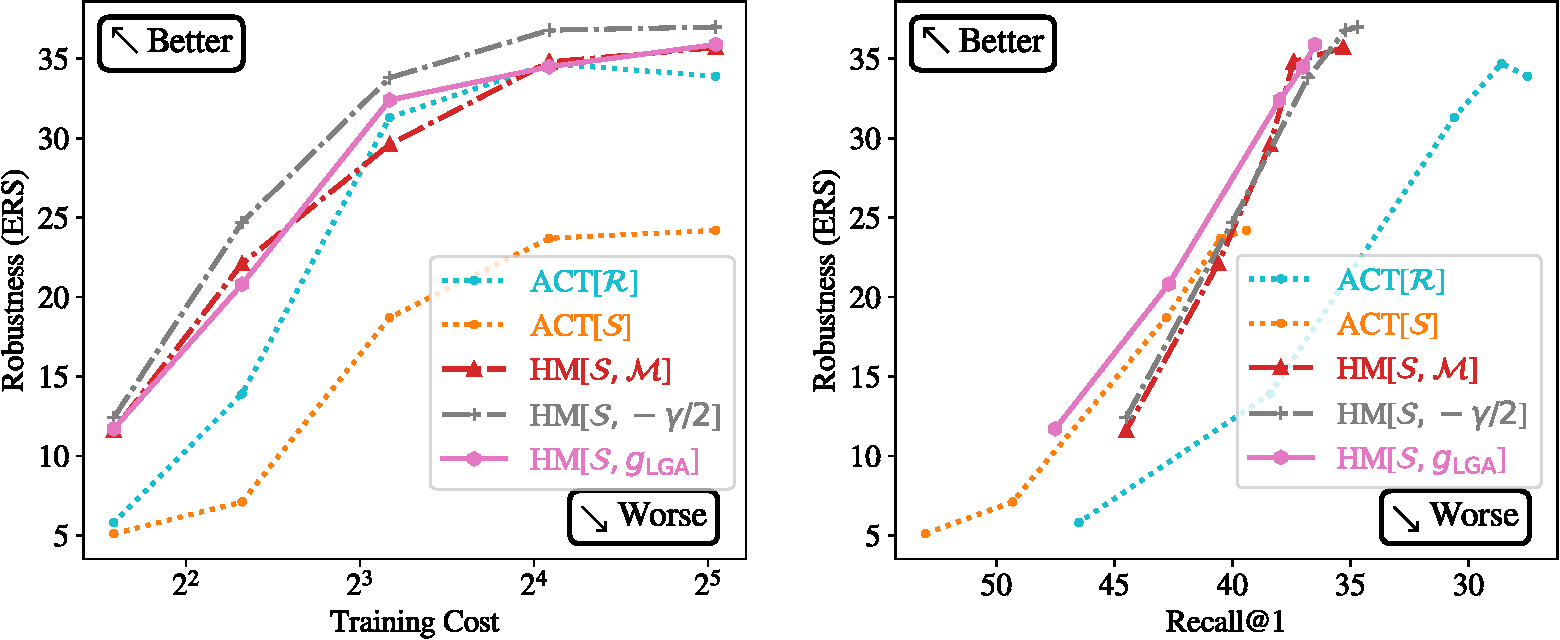
\includegraphics[width=\columnwidth]{figgaeff.pdf}
	\vspace{-1.9em}
	\caption{Performance of ``HM[$\mathcal{S},g_\mathsf{LGA}$]'' in
	\cref{tab:gaeff}.}
	\vspace{-1em}
	\label{fig:gaeff}
\end{figure}

\noindent\textbf{II. Gradual Adversary.}
%
HM[$\mathcal{S},\mathcal{M}$] may still
suffer from the imbalance between learning the embeddings and gaining
adversarial robustness as discussed in \cref{sec:32}.
%
Hence, we conduct further experiments %with an improved $H_\mathsf{D}$
following the discussion, as shown in \cref{tab:gaeff} and \cref{fig:gaeff}.
%
Compared to HM[$\mathcal{S},\mathcal{M}$], slightly boosting the hardness
with $g_\mathsf{B}(\cdot)$ benefits the ERS, but
results in a notably lower R@1;
%
A constant $H_\mathsf{D}$ at the upper bound of Semihard (\ie, $0$; too high
for both the early and the late phase of training) renders model collapse;
%
$H_\mathsf{D}$ at the lower bound (\ie, $-\gamma$; too low for the late phase)
leads to insignificant ERS improvement;
%
$H_\mathsf{D}{=}-\gamma/2$ provides a fair balance in training objectives, but
still suffers from inflexibility.
%
In contrast, being not susceptible to the mentioned problems of other choices,
HM[$\mathcal{S},g_\mathsf{LGA}$] achieves an ERS on par with
HM[$\mathcal{S},\mathcal{M}$], but is at the lowest R@1 performance penalty among all choices.
%
Its ERS is marginally lower than HM[$\mathcal{S},{-}\gamma/2$] because the
loss value eventually converges around ${-}\gamma/2$ due to optimization
difficulty, which means
adversarial triplets with $H_\mathsf{D}{\in}[{-}\gamma/2,0]$
are seldom created.

\begin{figure}[t]
	\vspace{-1.5em}
	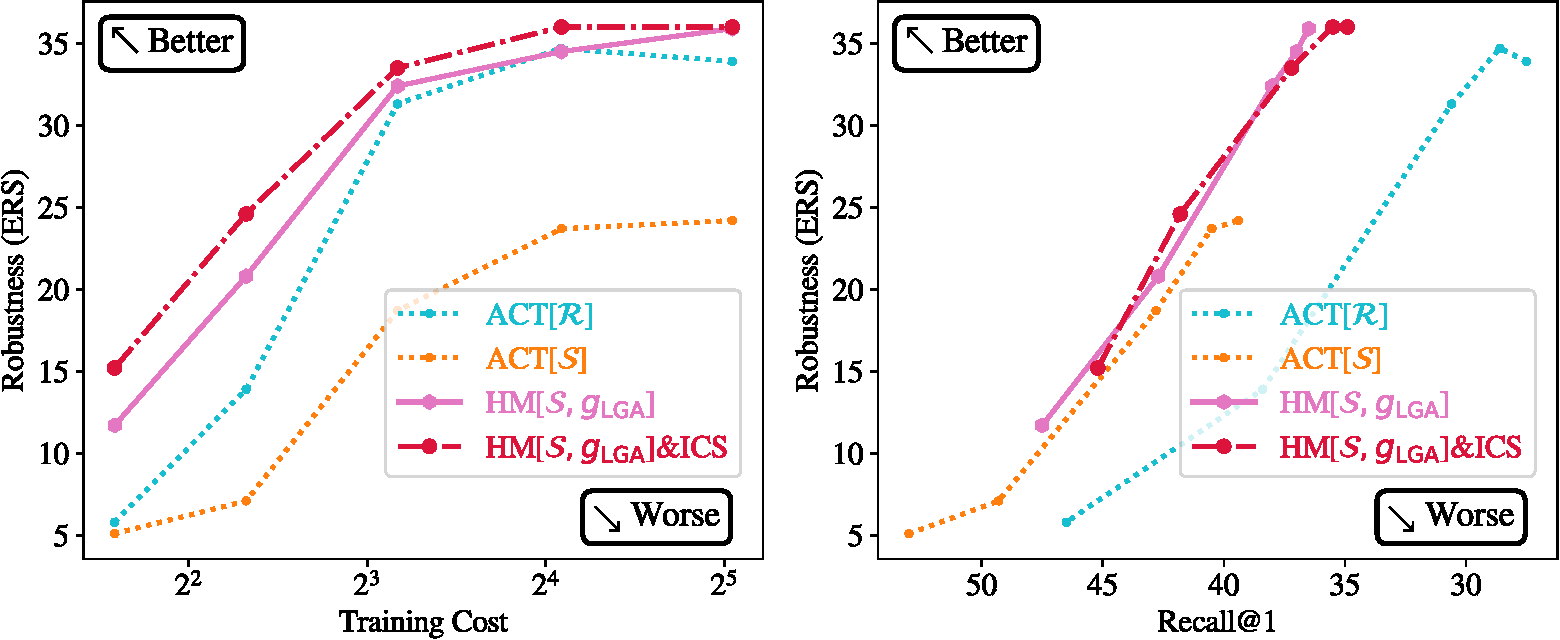
\includegraphics[width=\columnwidth]{figics.pdf}
	\vspace{-1.9em}
	\caption{Performance of ``HM[$\mathcal{S},g_\mathsf{LGA}$]\&ICS'' in \cref{tab:ics}.}
	\vspace{-1em}
	\label{fig:icscurve}
\end{figure}


\noindent\textbf{III. Intra-Class Structure.}
%
$L_\text{ICS}$ is independent to HM, but is incompatible with ACT as it does
not create adversarial anchor.
%
Thus, we validate this loss term with HM.
%
As shown in \cref{tab:ics} and \cref{fig:icscurve}, $L_\text{ICS}$ consistently
leads to a higher efficiency in gaining higher robustness at a low training
cost, while retaining an acceptable trade-off in R@1.

\noindent\textbf{IV. Summary.}
%
Eventually, HM[$\mathcal{S},g_\mathsf{LGA}$]\&ICS overwhelmingly outperforms
the state-of-the-art defense in robustness, training cost, and R@1 
performance, as shown in \cref{fig:introplot}.

\begin{table*}
\resizebox{\linewidth}{!}{
\setlength{\tabcolsep}{0.47em}
\renewcommand{\arraystretch}{1.05}%

\begin{tabular}{c|cc|cccc|ccccc|ccccc|c}

	\toprule

\multirow{2}{*}{\textbf{Dataset}} & \multicolumn{1}{c}{\multirow{2}{*}{\textbf{Defense}}} & \multirow{2}{*}{$\eta$} & \multicolumn{4}{c|}{\textbf{Benign Example}} & \multicolumn{10}{c|}{\textbf{White-Box Attacks for Robustness Evaluation}} & \multirow{2}{*}{\textbf{ERS$\uparrow$}}\tabularnewline
\cline{4-17} \cline{5-17} \cline{6-17} \cline{7-17} \cline{8-17} \cline{9-17} \cline{10-17} \cline{11-17} \cline{12-17} \cline{13-17} \cline{14-17} \cline{15-17} \cline{16-17} \cline{17-17}
 &  &  & R@1$\uparrow$ & R@2$\uparrow$ & mAP$\uparrow$ & NMI$\uparrow$ & CA+$\uparrow$ & CA-$\downarrow$ & QA+$\uparrow$ & QA-$\downarrow$ & TMA$\downarrow$ & ES:D$\downarrow$ & ES:R$\uparrow$ & LTM$\uparrow$ & GTM$\uparrow$ & GTT$\uparrow$ & \tabularnewline

	\midrule

\multirow{9}{*}{CUB} & N/A{[}$\mathcal{R}${]} & N/A & 53.9 & 66.4 & 26.1 & 59.5 & 0.0 & 100.0 & 0.0 & 99.9 & 0.883 & 1.762 & 0.0 & 0.0 & 14.1 & 0.0 & 3.8\tabularnewline
\cline{2-18} \cline{3-18} \cline{4-18} \cline{5-18} \cline{6-18} \cline{7-18} \cline{8-18} \cline{9-18} \cline{10-18} \cline{11-18} \cline{12-18} \cline{13-18} \cline{14-18} \cline{15-18} \cline{16-18} \cline{17-18} \cline{18-18} 
 & EST{[}$\mathcal{R}${]}~\cite{advrank} & 8 & 37.1 & 47.3 & 20.0 & 46.4 & 0.5 & 97.3 & 0.5 & 91.3 & 0.875 & 1.325 & 3.9 & 0.4 & 14.9 & 0.0 & 7.9\tabularnewline
 & ACT{[}$\mathcal{R}${]}~\cite{robrank} & 8 & 30.6 & 40.1 & 16.5 & 45.6 & 13.7 & 46.8 & 12.6 & 39.3 & 0.547 & 0.902 & 13.6 & 9.8 & 21.9 & 1.3 & 31.3\tabularnewline
 & HM{[}$\mathcal{S},g_{\mathsf{LGA}}${]} & 8 & 38.0 & 48.3 & 21.8 & 49.3 & 12.7 & 46.4 & 11.6 & 39.9 & 0.567 & 0.783 & 16.8 & 11.9 & 27.9 & 1.4 & 32.4\tabularnewline
 & HM{[}$\mathcal{S},g_{\mathsf{LGA}}${]}\&ICS & 8 & 37.2 & 47.8 & 21.4 & 48.4 & 12.9 & 40.9 & 14.7 & 33.7 & 0.806 & 0.487 & 17.1 & 13.2 & 26.3 & 2.3 & 33.5\tabularnewline
\cline{2-18} \cline{3-18} \cline{4-18} \cline{5-18} \cline{6-18} \cline{7-18} \cline{8-18} \cline{9-18} \cline{10-18} \cline{11-18} \cline{12-18} \cline{13-18} \cline{14-18} \cline{15-18} \cline{16-18} \cline{17-18} \cline{18-18} 
 & EST{[}$\mathcal{R}${]}~\cite{advrank} & 32 & 8.5 & 13.0 & 2.6 & 25.2 & 2.7 & 97.9 & 0.4 & 97.3 & 0.848 & 1.576 & 1.4 & 0.0 & 4.0 & 0.0 & 5.3\tabularnewline
 & ACT{[}$\mathcal{R}${]}~\cite{robrank} & 32 & 27.5 & 38.2 & 12.2 & 43.0 & 15.5 & 37.7 & 15.1 & 32.2 & 0.472 & 0.821 & 11.1 & 9.4 & 14.9 & 1.0 & 33.9\tabularnewline
 & HM{[}$\mathcal{S},g_{\mathsf{LGA}}${]} & 32 & 36.5 & 46.7 & 21.0 & 48.6 & 14.7 & 39.6 & 15.6 & 34.2 & 0.523 & 0.736 & 16.5 & 15.0 & 26.7 & 2.9 & 35.9\tabularnewline
 & HM{[}$\mathcal{S},g_{\mathsf{LGA}}${]}\&ICS & 32 & 34.9 & 45.0 & 19.8 & 47.1 & 15.5 & 37.7 & 16.6 & 30.9 & 0.753 & 0.506 & 17.9 & 16.7 & 27.3 & 2.9 & 36.0\tabularnewline

	\midrule 

\multirow{9}{*}{CARS} & N/A{[}$\mathcal{R}${]} & N/A & 62.5 & 74.0 & 23.8 & 57.0 & 0.2 & 100.0 & 0.1 & 99.6 & 0.874 & 1.816 & 0.0 & 0.0 & 13.4 & 0.0 & 3.6\tabularnewline
\cline{2-18} \cline{3-18} \cline{4-18} \cline{5-18} \cline{6-18} \cline{7-18} \cline{8-18} \cline{9-18} \cline{10-18} \cline{11-18} \cline{12-18} \cline{13-18} \cline{14-18} \cline{15-18} \cline{16-18} \cline{17-18} \cline{18-18} 
 & EST{[}$\mathcal{R}${]}~\cite{advrank} & 8 & 57.1 & 68.4 & 30.3 & 47.7 & 0.1 & 99.9 & 0.1 & 98.1 & 0.902 & 1.681 & 0.7 & 0.2 & 15.4 & 0.0 & 4.4\tabularnewline
 & ACT{[}$\mathcal{R}${]}~\cite{robrank} & 8 & 46.8 & 58.0 & 23.4 & 45.5 & 19.3 & 33.1 & 20.3 & 32.3 & 0.413 & 0.760 & 18.4 & 15.0 & 28.6 & 1.2 & 39.8\tabularnewline
 & HM{[}$\mathcal{S},g_{\mathsf{LGA}}${]} & 8 & 63.2 & 73.7 & 36.8 & 53.5 & 15.3 & 32.0 & 17.9 & 33.9 & 0.463 & 0.653 & 23.4 & 28.5 & 44.6 & 5.8 & 42.4\tabularnewline
 & HM{[}$\mathcal{S},g_{\mathsf{LGA}}${]}\&ICS & 8 & 61.7 & 72.6 & 35.5 & 51.8 & 21.0 & 23.3 & 23.1 & 22.2 & 0.698 & 0.415 & 31.2 & 38.0 & 47.8 & 9.6 & 47.9\tabularnewline
\cline{2-18} \cline{3-18} \cline{4-18} \cline{5-18} \cline{6-18} \cline{7-18} \cline{8-18} \cline{9-18} \cline{10-18} \cline{11-18} \cline{12-18} \cline{13-18} \cline{14-18} \cline{15-18} \cline{16-18} \cline{17-18} \cline{18-18} 
 & EST{[}$\mathcal{R}${]}~\cite{advrank} & 32 & 30.7 & 41.0 & 5.6 & 31.8 & 1.2 & 98.1 & 0.4 & 91.8 & 0.880 & 1.281 & 2.9 & 0.7 & 8.2 & 0.0 & 7.3\tabularnewline
 & ACT{[}$\mathcal{R}${]}~\cite{robrank} & 32 & 43.4 & 54.6 & 11.8 & 42.9 & 18.0 & 32.3 & 17.5 & 30.5 & 0.383 & 0.763 & 16.3 & 15.3 & 20.7 & 1.6 & 38.6\tabularnewline
 & HM{[}$\mathcal{S},g_{\mathsf{LGA}}${]} & 32 & 62.3 & 72.5 & 35.3 & 52.7 & 17.4 & 28.2 & 18.2 & 28.8 & 0.426 & 0.613 & 27.1 & 30.7 & 42.3 & 7.9 & 44.9\tabularnewline
 & HM{[}$\mathcal{S},g_{\mathsf{LGA}}${]}\&ICS & 32 & 60.2 & 71.6 & 33.9 & 51.2 & 19.3 & 25.9 & 19.6 & 25.7 & 0.650 & 0.446 & 30.3 & 36.7 & 46.0 & 8.8 & 46.0\tabularnewline

	\midrule

\multirow{9}{*}{SOP} & N/A{[}$\mathcal{R}${]} & N/A & 62.9 & 68.5 & 39.2 & 87.4 & 0.1 & 99.3 & 0.2 & 99.1 & 0.845 & 1.685 & 0.0 & 0.0 & 6.3 & 0.0 & 4.0\tabularnewline
\cline{2-18} \cline{3-18} \cline{4-18} \cline{5-18} \cline{6-18} \cline{7-18} \cline{8-18} \cline{9-18} \cline{10-18} \cline{11-18} \cline{12-18} \cline{13-18} \cline{14-18} \cline{15-18} \cline{16-18} \cline{17-18} \cline{18-18} 
 & EST{[}$\mathcal{R}${]}~\cite{advrank} & 8 & 52.7 & 58.5 & 14.8 & 85.7 & 6.4 & 69.7 & 3.9 & 64.6 & 0.611 & 1.053 & 3.8 & 2.2 & 10.2 & 1.3 & 19.0\tabularnewline
 & ACT{[}$\mathcal{R}${]}~\cite{robrank} & 8 & \uline{45.1} & \uline{50.2} & \uline{11.5} & \uline{84.7} & \uline{27.0} & \uline{10.2} & \uline{27.0} & \uline{7.9} & \uline{0.285} & \uline{0.483} & \uline{15.6} & \uline{16.1} & \uline{23.9} & \uline{10.7} & \uline{50.3}\tabularnewline
 & HM{[}$\mathcal{S},g_{\mathsf{LGA}}${]} & 8 & 49.0 & 54.1 & 12.7 & 85.0 & 29.9 & 4.7 & 31.6 & 3.6 & 0.455 & 0.283 & 39.3 & 40.9 & 38.8 & 43.0 & 61.7\tabularnewline
 & HM{[}$\mathcal{S},g_{\mathsf{LGA}}${]}\&ICS & 8 & 47.7 & 52.7 & 12.2 & 84.8 & 30.6 & 4.7 & 31.2 & 3.5 & 0.466 & 0.266 & 38.6 & 40.3 & 38.6 & 44.3 & 61.8\tabularnewline
\cline{2-18} \cline{3-18} \cline{4-18} \cline{5-18} \cline{6-18} \cline{7-18} \cline{8-18} \cline{9-18} \cline{10-18} \cline{11-18} \cline{12-18} \cline{13-18} \cline{14-18} \cline{15-18} \cline{16-18} \cline{17-18} \cline{18-18} 
 & EST{[}$\mathcal{R}${]}~\cite{advrank} & 32 & 46.0 & 51.4 & 24.5 & 84.7 & 12.5 & 43.6 & 10.6 & 34.8 & 0.468 & 0.830 & 9.6 & 7.2 & 17.3 & 3.8 & 31.7\tabularnewline
 & ACT{[}$\mathcal{R}${]}~\cite{robrank} & 32 & 47.5 & 52.6 & 25.5 & 84.9 & 24.1 & 10.5 & 22.7 & 9.4 & 0.253 & 0.532 & 21.2 & 21.6 & 27.8 & 15.3 & 50.8\tabularnewline
 & HM{[}$\mathcal{S},g_{\mathsf{LGA}}${]} & 32 & 47.7 & 52.7 & 25.3 & 84.8 & 30.6 & 4.7 & 31.2 & 3.5 & 0.466 & 0.266 & 38.6 & 40.3 & 38.6 & 44.3 & 61.8\tabularnewline
 & HM{[}$\mathcal{S},g_{\mathsf{LGA}}${]}\&ICS & 32 & T:V &  &  &  &  &  &  &  &  &  &  &  &  &  & \tabularnewline

	\bottomrule

\end{tabular}}
	\vspace{-0.5em}
\caption{Comparison of Our Defense to State-of-The-Art Methods on Commonly Used DML Datasets.}
	\label{tab:sota}
\end{table*}


\subsection{Comparison to State-of-The-Art Defense}
\label{sec:43}

After validating the effectiveness of our proposed method, we conduct
experiments on CUB, CARS and SOP to compare our proposed method
with the state-of-the-art defense methods, \ie, EST~\cite{advrank}
and ACT~\cite{robrank}. The corresponding results are shown in \cref{tab:sota}.
%
An ideal defense method should be able to achieve a high ERS and a high R@1
at a low training cost (\ie, $\eta+1$).
%
The ability of a method to achieve a high ERS under a low training cost
indicates a high efficiency.

According to the results, EST[$\mathcal{R}$] achieves a relatively high R@1
when $\eta{=}8$, but suffers from a drastic drop in R@1 when $\eta$ is
increased to $32$.
%
Nevertheless, EST[$\mathcal{R}$] only lead to a moderate robustness
compared to other methods.
%
Experiments for EST[$\mathcal{S}$] are omitted as EST has been greatly
outperformed by ACT~\cite{robrank}, and it is expected to result in
even lower ERS based on the observations in previous subsections.
%
Although ACT[$\mathcal{R}$] achieves a relatively high ERS, its R@1 performance
drop is distinct on every dataset.
%
According the previous subsections, ACT[$\mathcal{S}$] can lead to a high R@1,
but along with a significantly lower ERS.
%
Thus, results for ACT[$\mathcal{S}$] are omitted for being insufficiently robust.

Our method overwhelmingly outperforms the previous methods in terms of the
overall performance. Namely, our method achieves the highest ERS with a very
low decrement in R@1 under a fixed training cost.
%
HM[$\mathcal{R},\mathcal{M}$] or HM[$\mathcal{R},g_\mathsf{LGA}$] can reach an
even higher ERS, but are excluded from comparison due to significant drop in
R@1.
%

It \emph{must} be acknowledged that the high R@1 performance of our method
largely stems from the source triplet sampling strategy, \ie, Softhard, instead
of our contribution.
%
Nevertheless, the state-of-the-art method, \ie, ACT could not reach the same
level of robustness with the same sampling strategy.

It \emph{should} be noted that the $L_\text{ICS}$ term improves 
robustness against most attacks involved in ERS, but also increases the
tendency to collapse (observed during TMA~\cite{flowertower} attack --
high cosine similarity between two arbitrary benign examples).
%
In some cases (\eg, on SOP), the performance drop \emph{w.r.t} TMA may
neutralize the ERS gain from other attacks.

Conclusively, being selective on both benign and
adversarial training samples is crucial for preventing model collapse, and
achieving good performance on both types of samples.
%
HM is a flexible tool for specifying such ``selection'' of adversarial
examples, while LGA can be interpreted as a concrete ``selection''.
%
ICS loss further exploits the given sextuplet.

Further analysis, technical details, and limitations, \etc,
are presented in the supplementary document.


\section{Conclusion}
\label{sec:5}

%Adversarial robustness is crucial for applications.
%
In this paper, HM efficiently and flexibly creates adversarial examples for
adversarial training;
%
LGA specifies an ``intermediate'' destination hardness for balancing robustness
and performance on benign examples;
%
ICS loss term further improves model robustness.
%
The state-of-the-art defenses have been surpassed in terms of overall performance.

%%%%%%%%% REFERENCES
{\small
\bibliographystyle{ieee_fullname}
\bibliography{egbib}
}

%\newpage
\appendix

\section{My Memo}

\subsection{To be investigated}

\begin{itemize}

	\item [*] re-design Gradual Adversary for HM based on that for the amdsemi. |
		\[
			(1-\frac{\text{prev\_loss}|_0^{2+\beta}}{2+\beta}) \times
			(\phi - H_\text{dst})\mathbb{I}\{\phi > H_\text{dst}\}
		\]
		So that for triplets that are not hard enoguh, when
		$prevloss \rightarrow 0$, $E[H_\text{dst}]\rightarrow \phi$.
	
	\item [!] difference between EST, ACT, AMD/ AMDsemi.
		Other methods (than HM) cannot effectively learn from the strongest
		adversary as the inner maximization is indirectly (and not guaranteed).
		HM follows the min-max paradigm (can be incorporated into FAT etc).
		Both ACT and HM stops at a specific point.
	
	\item [?] does the new generic HM work under FAT?

	\item [?] benchmark other metric learning loss functions for adversarial
		training. Can HM or GradualAdversary be adopted for other loss functions?

	\item [*] Sampling also matters in adversarial training for deep metric learning.

		[source hardness and destination hardness] different source sampling
		strategy and different destination sampling strategy. attack
		destination. DML loss not that sensitive to sampling? or generic
		advtrain method for DML? | still investigating

	\item [*] 7-step PGD (as well as 16-step PGD) and better aligned comparison:
		compare when these methods reach similar retrieval performance.
		Meanwhile we can do experiments much faster.

	\item Adversarial training (does not allow any distance moving) may
		encourage collapse (a trivial solution to the requirement). What if we
		loosen the requirement and convert it into a new constraint? For
		instance, \[
			L_{loosen}(a,p,n)=L_{base}(a,p,n)+\lambda_{1}L(a,\tilde{a},p)+\lambda_{2}L_{triplet}(a,\tilde{a},n)
		\] where the $L_{base}$ can be either $L_{triplet}$, $L_{rest}$, or
		$L_{act}$. Question: should we do this for every sample? i.e., \[
			L_{loosen}(a,p,n)=L_{base}(a,p,n)+\sum_{x\in\{a,p,n\}}L(x,\tilde{x},n_{x})
		\]

	\item [?] adversarial training that does not allow embedding move may
		encourage model collapse. Maybe we just apply some loosened restrction
		such as aap? i.e. $(a,\tilde{a},p;\gamma=0)$.

	\item ?  what about other types of metric learining loss functions? |
		investigating (we first make the most classical method work)

	\item ?  effectiveness of AMD Semi is to be verified. | as effective
		as ACT, reaches slightly higher ERS. But performs worse than ACT on
		some attacks, while performs better one some other attacks. | needs to
		be interpreted.

	\item ? can we learn a good destination distribution? | too
		complicated? not necessary currently.

	\item 1. APGD as the optimization algorithm? | postpone

	\item 1. ? mixing amdsemi and act for adversarial training. They are good
		at different aspects.

	\item verify model collapse

	\item [?] Combine and even better. | Mixing ACT and AMDsemi does result
		in clearly better results. It's on par with AMDsemi. Are they really
		that different?

\end{itemize}


\subsection{Done, Discarded or Rejected}

\begin{enumerate}

	\item [\cmark] revise HM. align dap dan directly instead of the loss.

	\item [\cmark] \checkmark dynamically changing schedule for amdsemi? |
		looks good | the sqrt scheme works the best. (gradually increasing the
		hardness makes sense)

	\item [\cmark] (codecheck) does amd really honour the pgditer parameter? |
		direct adoptation of madry defense is really prone to model collapse.

	\item [\xmark] MSE attack? | TMA is already close enough to it.

	\item [\xmark] Faster training (algorithm tweak) based FAT/other | this is
		a dead end. ACT has a different loss function to the outer minimization
		problem, and hence result in different gradient and we cannot reuse
		these gradients for algorithms like free adversarial training.
		Re-calculating the gradients we need would simple double the
		computational cost of the algorithm and diminish the gain from Free
		Adversarial Training. We are no longer using the core benefit of FAT in
		this way. In contrast, the AMD / AMDhm formulation can benefit from
		this setup. | Further experiments suggest very weak robustness and the
		models are very prone to collapse due to the non-zero initial delta
		(results in too hard adversarial example).  | gradient approximation
		does not look convincing. triplet gradient and ACT gradient does not
		look convertible.

	\item [\cmark] implement FAT for faster exp iteration | works on toy
		dataset. too prone to collapse. if we try to avoid model collapse, the
		adversarial robustness will decrease significantly.

	\item [\cmark] what if we use stopat for RAMD? | similar effect to amdsemi.
		misguiding gradient does not significantly affect AMD defense. So it
		is not quite necessary.
	
\end{enumerate}


\end{document}
